\documentclass[a4paper,11pt]{report}
\usepackage[T1]{fontenc}
\usepackage[utf8]{inputenc}
\usepackage{lmodern}
\usepackage{graphicx}
\usepackage{url}
\usepackage{parskip}
\usepackage{pmboxdraw}

% margins
\usepackage[top=2cm, bottom=3cm, left=3.8cm, right=3.8cm]{geometry}

% PDF file properties and links
\usepackage{hyperref}
\hypersetup{
  pdfauthor = {Sébastien Wilmet},
  pdftitle = {The GLib/GTK+ Development Platform},
  pdfcreator = {Texlive},
  pdfproducer = {Texlive},
  %colorlinks = false,
  pdfborder = 0 0 0
}

% Another package for code syntax highlighting is minted. By default minted has better colors for reading the document on a screen, but I think it is possible to have decent colors with listings too, it just requires more configuration. For printing purposes (without colors), I think listings is better. And this document is meant to be printed.
\usepackage{listings}
\lstset{
  language=C,
  basicstyle={\small\ttfamily},
  basewidth=0.5em,
  showstringspaces=false,
  captionpos=b
%   floatplacement=htbp
% Frames look nice, but it should be used cautiously. A frame around something means that the "something" is important. A frame will maybe be used later in this book to give a summary of important things. If each piece of code is surrounded by a frame, the important text will not be as highlighted as it should.
%   frame=single,
%   frame=tb,
% Will be useful later for large piece of code (create a new environment named lstlistinglarge or something like that).
%   linewidth=15cm,
%   xleftmargin=-1cm,
%   xrightmargin=-1cm
}

\lstloadlanguages{C, C++, Lisp, bash}

% Separate listings from the text (recommended in the Listings doc, instead of using frames).
% But with captions at the bottom, it is not very useful.
%\newcommand{\topfigrule}{\hrule\kern-0.4pt\relax}
%\newcommand{\botfigrule}{\hrule\kern-0.4pt\relax}

\newcommand{\shellcmd}[1]{\texttt{#1}}

\newcommand{\bookversion}{0.7}

\title{The GLib/GTK+ Development Platform\\[0.3cm]
{\normalsize A Getting Started Guide}\\[0.3cm]
{\normalsize Version \bookversion}}

\author{Sébastien Wilmet}

\begin{document}

\maketitle
\tableofcontents

\chapter{Introduction}

This text is a guide to get started with the GLib/GTK+ development platform, with the C language. It is sometimes assumed that the reader uses a Unix-like system.

Warning: this ``book'' is far from finished, you're reading the version~\bookversion. If you have any comments, don't hesitate to contact me at \url{swilmet@gnome.org}, thanks!

The sources of this book are available at:\\
\url{https://github.com/swilmet/glib-gtk-book}

\section{License}
\label{intro-license}

\begin{center}
  \includegraphics[height=0.8cm]{images/creative-commons.pdf}
\end{center}

This work is licensed under a Creative Commons Attribution-ShareAlike 4.0 International License:\\
\url{https://creativecommons.org/licenses/by-sa/4.0/}

Some sections are based on the book \emph{GTK+/Gnome Application Development}, by Havoc Pennington, written in 1999, edited by the New Riders Publishing, and licensed under the Open Publication License. The latest version of the Open Publication License can be found at:\\
\url{http://www.opencontent.org/openpub/}

\section{What is GLib and GTK+?}

Roughly speaking, GLib is a set of libraries: GLib core, GObject and GIO. Those three libraries are developed in the same Git repository called \emph{glib}, so when referring to ``GLib'', it can either mean ``GLib core'' or the broader set including also GObject and GIO.

GLib core provides data structure handling for C (linked lists, trees, hash tables, …), portability wrappers, an event loop, threads, dynamic loading of modules and lots of utility functions.

GObject -- which depends on GLib core -- simplifies the object-oriented programming and event-driven programming paradigms in C. Event-driven programming is not only useful for graphical user interfaces (with user events such as key presses and mouse clicks), but also for daemons that respond to hardware changes (a USB stick inserted, a second monitor connected, a printer low on paper), or software that listen to network connections or messages from other processes, and so on.

GIO -- which depends on GLib core and GObject -- provides high-level APIs for input/output: reading a local file, a remote file, a network stream, inter-process communication with D-Bus, and many more.

The GLib libraries can be used to write operating system services, libraries, command line utilities and such. GLib offers higher-level APIs than the POSIX standard; it is therefore more comfortable to write a C program with GLib.

GTK+ is a widget toolkit based on GLib that can be used to develop applications with a graphical user interface (GUI). The first version of GTK+, or the GIMP Tool Kit\footnote{The name ``The GIMP Tool Kit'' is now rarely used, today it is more commonly known as GTK+ for short.}, was mainly written by Peter~Mattis in 1996 for the GIMP (GNU Image Manipulation Program), but has quickly become a general-purpose library. The ``+'' has been added later to distinguish between the original version and a new version that added object oriented features. GLib started as part of GTK+, but is now a standalone library.

The GLib and GTK+ APIs are documented with GTK-Doc. Special comments are written in the source code, and GTK-Doc extracts those comments to generate HTML pages.

Although GLib and GTK+ are written in C, language bindings are available for JavaScript, Python, Perl and many other programming languages. At the beginning, manual bindings were created, which needed to be updated each time the API of the library changed. Nowadays the language bindings are generic and are thus automatically updated when, for example, new functions are added. This is thanks to GObject Introspection. Special annotations are added to the GTK-Doc comments, to expose more information than what the C syntax can provide, for example about ownership transfer of dynamically-allocated content\footnote{For example, whether you need to free the return value.}. Any C library with GObject Introspection support is thus available from many programming languages. In addition, the annotations are also useful to the C programmer because it's a good and succint way to document certain recurrent API aspects.

GLib and GTK+ are part of the GNU Project, whose overall goal is developing a free operating system (named GNU) plus applications to go with it. GNU stands for ``GNU's Not Unix'', a humorous way of saying that the GNU operating system is Unix-compatible. You can learn more about GNU at \url{https://www.gnu.org}.

The GLib/GTK+ web site is: \url{http://www.gtk.org}

\section{The GNOME Desktop}

An important project for GLib and GTK+ is GNOME. GNOME, which is also part of GNU, is a free/libre desktop environment started in 1997 by Miguel~de~Icaza and Federico~Mena-Quintero. GNOME makes extensive use of GTK+, and the latter is now developed primarily by GNOME developers.

``GNOME'' is actually an acronym: GNU Network Object Model Environment\footnote{As for GTK+, the complete name of GNOME is rarely used and doesn't reflect today's reality.}. Originally, the project was intended to create a framework for application objects, similar to Microsoft's OLE and COM technologies. However, the scope of the project rapidly expanded; it became clear that substantial groundwork was required before the ``network object'' part of the name could become reality. Old versions of GNOME included an object embedding architecture called Bonobo, and GNOME~1.0 included a fast, light CORBA ORB called ORBit. Bonobo has been replaced by D-Bus, an inter-process communication system.

GNOME has two important faces. From the user's perspective, it is an integrated desktop environment and application suite. From the programmer's perspective, it is an application development framework (made up of numerous useful libraries that are based on GLib and GTK+). Applications written with the GNOME libraries run fine even if the user isn't running the desktop environment, but they integrate nicely with the GNOME desktop if it's available.

The desktop environment includes a ``shell'' for task switching and launching programs, a ``control center'' for configuration, lots of applications such as a file manager, a web browser, a movie player, etc. These programs hide the traditional Unix command line behind an easy-to-use graphical interface.

GNOME's development framework makes it possible to write consistent, easy-to-use, interoperable applications. The designers of windowing systems such as X11 or Wayland made a deliberate decision not to impose any user interface policy on developers; GNOME adds a ``policy layer,'' creating a consistent look-and-feel. Finished GNOME applications work well with the GNOME desktop, but can also be used ``standalone'' -- users only need to install GNOME's shared libraries. A GNOME application isn't tied to a specific windowing system, GTK+ provides backends for the X Window System, Wayland, Mac OS X, Windows, and even for a web browser.

At the time of writing, there are new GLib, GTK+ and GNOME stable releases every six months, around March and September. A version number has the form ``\texttt{major.minor.micro}'', where ``\texttt{minor}'' is even for stable versions and is odd for unstable versions. For example, the 3.18.* versions are stable, but the 3.19.* versions are unstable. A new micro stable version (e.g. 3.18.0 $\rightarrow$ 3.18.1) doesn't add new features, only translation updates, bug fixes and performance improvements. GNOME components are meant to be installed with the same versions, alongside the version of GTK+ and GLib released at the same time; it's for instance a bad idea to run a GNOME daemon in version 3.18 with the control center in version 3.16. At the time of writing, the latest stable versions are: GLib~2.46, GTK+~3.18 and GNOME~3.18, all released at the same time in September 2015. For a library, a new major version number usually means there has been an API break, but thankfully previous major versions are parallel-installable with the new version. During a development cycle (e.g. 3.19), there is no API stability guarantees for \emph{new} features; but by being an early adopter your comments are useful to discover more quickly design flaws and bugs.

More information about GNOME: \url{https://www.gnome.org/}

\section{Prerequisites}

This book assumes that you already have some programming practice. Here is a list of recommended prerequisites, with book references.

\begin{itemize}
  \item This text supposes that you already know the C language. The reference book is \emph{The C Programming Language}, by Brian~Kernighan and Dennis~Ritchie \cite{k-r-book}.

  \item Object-oriented programming (OOP) is also required for learning GObject. You should be familiar with concepts like inheritance, an interface, a virtual method or polymorphism. A good book, with more than sixty guidelines, is \emph{Object-Oriented Design Heuristics}, by Arthur~Riel \cite{oop-book}.

  \item Having read a book on data structures and algorithms is useful, but you can learn that in parallel. A recommended book is \emph{The Algorithm Design Manual}, by Steven~Skiena \cite{algo-book}.

  \item If you want to develop your software on a Unix-like system, another prerequisite is to know how Unix works, and be familiar with the command line, a bit of shell scripting and how to write a Makefile. A possible book is \emph{UNIX for the Impatient}, by Paul~Abrahams \cite{unix-impatient}.

  \item Not strictly required, but highly recommended is to use a version control system like Git. A good book is \emph{Pro Git}, by Scott~Chacon \cite{pro-git}.
\end{itemize}

\section{Why and When Using the C Language?}

The GLib and GTK+ libraries can be used by other programming languages than C. Thanks to GObject Introspection, automatic bindings are available for a variety of languages for all libraries based on GObject. Official GNOME bindings are available for the following languages: C++, JavaScript, Perl, Python and Vala\footnote{\url{https://wiki.gnome.org/Projects/Vala}}. Vala is a new programming language based on GObject which integrates the peculiarities of GObject directly in its C\#-like syntax. Beyond the official GNOME bindings, GLib and GTK+ can be used in more than a dozen other programming languages, with a varying level of support. So why and when choosing the C language? For writing a daemon on a Unix system, C is the \emph{de facto} language. But it is less obvious for an application. To answer the question, let's first look at how to structure an application codebase.

% Adapted from a FAQ question in GGAD.
\subsection{Separate the Backend from the Frontend}
\label{intro-backend-frontend-separation}
A good practice is to separate the graphical user interface from the rest of the application. For a variety of reasons, an application's graphical interface tends to be an exceptionally volatile and ever-changing piece of software. It's the focus of most user requests for change. It is difficult to plan and execute well the first time around -- often you will discover that some aspect of it is unpleasant to use only after you have written it. Having several different user interfaces is sometimes desirable, for example a command-line version, or a web-based interface.

In practical terms, this means that any large application should have a radical separation between its various \emph{frontends}, or interfaces, and the \emph{backend}. The backend should contain all the ``hard parts'': your algorithms and data structures, the real work done by the application. Think of it as an abstract ``model'' being displayed to and manipulated by the user.

Each frontend should be a ``view'' and a ``controller.'' As a ``view,'' the frontend must note any changes in the backend, and change the display accordingly. As a ``controller,'' the frontend must allow the user to relay requests for change to the backend (it defines how manipulations of the frontend translate into changes in the model).

There are many ways to discipline yourself to keep your application separated. A couple of useful ideas:
\begin{itemize}
  \item Write the backend as a library. At the beginning the library can be internal to the application and statically linked, without API/ABI stability guarantees. When the project grows up, and if the code is useful for other programs, you can turn easily your backend into a shared library.
  \item Write at least two frontends from the start; one or both can be ugly prototypes, you just want to get an idea how to structure the backend. Remember, frontends should be easy; the backend has the hard parts.
\end{itemize}

The C language is a good choice for the backend part of an application. By using GObject and GObject Introspection, your library will be available for other projects written in various programming languages. On the other hand, a Python or JavaScript library cannot be used in other languages. For the frontend(s), a higher-level language may be more convenient, depending on what languages you already are proficient with.

\subsection{Other Aspects to Keep in Mind}
If you're hesitant about the language to choose, here are other aspects to keep in mind. Note that this text is a little biased since the C language has been chosen.

C is a static-typed language: the variable types and function prototypes in a program are all known at compilation time. Lots of trivial errors are discovered by the compiler, such as a typo in a function name. The compiler is also a great help when doing code refactorings, which is essential for the long-term maintainability of a program. For example when you split a class in two, if the code using the initial class is not updated correctly, the compiler will kindly tell you so\footnote{Well, \emph{kindly} is perhaps not the best description, spewing out loads of errors is closer to reality.}. With test-driven development (TDD), and by writing unit tests for \emph{everything}, writing a huge codebase in a dynamic-typed language like Python is also feasible. With a very good code coverage, the unit tests will also detect errors when refactoring the code. But unit tests can be much slower to execute than compiling the code, since it tests also the program behavior. So it's maybe not convenient to run all unit tests when doing code refactorings. Of course writing unit tests is also a good practice for a C codebase! However for the GUI part of the code, writing unit tests is often not a high-priority task if the application is well tested by its developers.

C is an explicit-typed language: the variable types are visible in the code. It is a way to self-document the code; you usually don't need to add comments to explain what the variables contain. Knowing the type of a variable is important to understand the code, to know what the variable represents and what functions can be called on it. On a related matter, the \emph{self} object is passed explicitly as a function argument. Thus when an attribute is accessed through the \emph{self} pointer, you know where the attribute comes from. Some object-oriented languages have the \emph{this} keyword for that purpose, but it is sometimes optional like in C++ or Java. In this latter case, a useful text editor feature is to highlight differently attributes, so even when the \emph{this} keyword is not used, you know that it's an attribute and not a local variable. With the \emph{self} object passed as an argument, there is no possible confusions.

The C language has a very good \emph{toolchain}: stable compilers (GCC, Clang, …), text editors (Vim, Emacs, …), debuggers (GDB, Valgrind, …), static-analysis tools, ...

For some programs, a garbage collector is not appropriate because it pauses the program regularly to release unused memory. For critical code sections, such as real-time animations, it is not desirable to pause the program (a garbage collector can sometimes run during several seconds). In this case, manual memory management like in C is a solution.

Less important, but still useful; the verbosity of C in combination with the GLib/GTK+ conventions has an advantage: the code can be searched easily with a command like \shellcmd{grep}. For example the function \lstinline{gtk_widget_show()} contains the namespace (\lstinline{gtk}), the class (\lstinline{widget}) and the method (\lstinline{show}). With an object-oriented language, the syntax is generally \lstinline[language=C++]{object.show()}. If ``show'' is searched in the code, there will most probably be more false positives, so a smarter tool is needed. Another advantage is that knowing the namespace and the class of a method can be useful when reading the code, it is another form of self-documentation.

More importantly, the GLib/GTK+ API documentation is primarily written for the C language. Reading the C documentation while programming in another language is not convenient. Some tools are currently in development to generate the API documentation for other target languages, so hopefully in the future it won't be a problem anymore.

GLib/GTK+ are themselves written in C. So when programming in C, there is no extra layer. An extra layer is potentially a source of additional bugs and maintenance burdens. Moreover, using the C language is probably better for pedagogical purposes. A higher-level language can hide some details about GLib/GTK+. So the code is shorter, but when you have a problem you need to understand not only how the library feature works, but also how the language binding works.

That said, if (1) you're not comfortable in C, (2) you're already proficient with a higher-level language with GObject Introspection support, (3) you plan to write just a small application or plugin, then choosing the higher-level language makes perfect sense.

\section{Learning Path}
\label{intro-learning-path}
%TODO when the book is finished, rename this section as "Structure of the Book"

Normally this section should be named ``Structure of the Book'', but as you can see the book is far from finished, so instead the section is named ``Learning Path''.

The logical learning path is:
\begin{enumerate}
  \item The bases of GLib core;
  \item Object-Oriented Programming in C and the bases of GObject;
  \item GTK+ and GIO in parallel.
\end{enumerate}

Since GTK+ is based on GLib and GObject, it is better to understand the bases of those two libraries first. Some tutorials dive directly into GTK+, so after a short period of time you can display a window with some text and three buttons; it's fun, but knowing GLib and GObject is not a luxury if you want to understand what you're doing, and a realistic GTK+ application extensively uses the GLib libraries. GTK+ and GIO can be learned in parallel --- once you start using GTK+, you will see that some non-GUI parts are based on GIO.

So this book begins with the GLib core library (chapter~\ref{glib} p.~\pageref{glib}), then introduces Object-Oriented Programming in C (chapter~\ref{oop} p.~\pageref{oop}) followed by a Further Reading chapter (p.~\pageref{further-reading}).

\section{The Development Environment}
\label{intro-dev-environment}

This section describes the development environment typically used when programming with GLib and GTK+ on a Unix system.

On a GNU/Linux distribution, a single package or group can often be installed to get a full C development environment, including, but not limited to:
\begin{itemize}
  \item a C89-compatible compiler, GCC for instance;
  \item the GNU debugger GDB;
  \item GNU Make;
  \item the Autotools (Autoconf, Automake and Libtool);
  \item the man-pages of: the Linux kernel and the glibc\footnote{Do not confuse the GNU C Library (glibc) with GLib. The former is lower-level.}.
\end{itemize}

For using GLib and GTK+ as a developer, there are several solutions:
\begin{itemize}
  \item The headers and the documentation can be installed with the package manager. The name of the packages end typically with one of the following suffixes: \texttt{-devel}, \texttt{-dev} or \texttt{-doc}. For example \texttt{glib2-devel} and \texttt{glib2-doc} on Fedora.
  \item The latest versions of GLib and GTK+ can be installed with Jhbuild:\\
  \url{https://wiki.gnome.org/Projects/Jhbuild}
\end{itemize}

To read the API documentation of GLib and GTK+, Devhelp is a handy application, if you have installed the \texttt{-dev} or \texttt{-doc} package. For the text editor or IDE, there are many choices (and a source of many trolls): Vim, Emacs, gedit, Anjuta, MonoDevelop/Xamarin Studio, Geany, … A promising specialized IDE for GNOME is Builder, currently in development. For creating a GUI with GTK+, you can either write directly the code to do it, or you can use Glade to design the GUI graphically. Finally, GTK-Doc is used for writing API documentation and add the GObject Introspection annotations.

When using GLib or GTK+, pay attention to not use deprecated APIs for newly-written code. Be sure that you read the latest documentations. They are also available online at:\\
\url{https://developer.gnome.org/}

\section{Acknowledgments}

Thanks to: Christian Stadelmann, Errol van~de~l'Isle and Andrew Colin Kissa.

\chapter{GLib, the Core Library}
\label{glib}

GLib is the low-level core library that forms the basis for projects such as GTK+ and GNOME. It provides data structures, utility functions, portability wrappers, and other essential functionality such as an event loop and threads. GLib is available on most Unix-like systems and Windows.

This chapter covers some of the most commonly-used features. GLib is simple, and the concepts are familiar; so we'll move quickly. For more complete coverage of GLib, see the latest API documentation that comes with the library (for the development environment, see section~\ref{intro-dev-environment} on p.~\pageref{intro-dev-environment}). By the way: if you have very specific questions about the implementation, don't be afraid to look at the source code. Normally the documentation contains enough information, but if you come across a missing detail, please file a bug (of course, the best would be with a provided patch).

GLib's various facilities are intended to have a consistent interface; the coding style is semi-object-oriented, and identifiers are prefixed with ``g'' to create a kind of namespace.

GLib has a few toplevel headers:
\begin{itemize}
  \item \header{glib.h}, the main header;
  \item \header{gmodule.h} for dynamic loading of modules;
  \item \header{glib-unix.h} for Unix-specific APIs;
  \item \header{glib/gi18n.h} and \header{glib/gi18n-lib.h} for internationalization;
  \item \header{glib/gprintf.h} and \header{glib/gstdio.h} to avoid pulling in all of stdio.
\end{itemize}

\bigskip
Note: instead of reinventing the wheel, this chapter is heavily based on the corresponding chapter in the book \emph{GTK+/Gnome Application Development} by Havoc Pennington, licensed under the Open Publication License (see section~\ref{intro-license} p.~\pageref{intro-license}). GLib has a very stable API. Despite the fact that Havoc Pennington's book was written in 1999 (for GLib~1.2), only a few updates were required to fit the latest GLib versions (version~2.42 at the time of writing).

\section{Basics}

GLib provides substitutes for many standard and commonly-used C language constructs. This section describes GLib's fundamental type definitions, macros, memory allocation routines, and string utility functions.

\subsection{Type Definitions}

Rather than using C's standard types (\lstinline{int}, \lstinline{long}, etc.) GLib defines its own. These serve a variety of purposes. For example, \lstinline{gint32} is guaranteed to be 32 bits wide, something no standard C89 type can ensure. \lstinline{guint} is simply easier to type than \lstinline{unsigned}. A few of the typedefs exist only for consistency; for example, \lstinline{gchar} is always equivalent to the standard \lstinline{char}.

The most important primitive types defined by GLib:
\begin{itemize}
  \item \lstinline{gint8}, \lstinline{guint8}, \lstinline{gint16}, \lstinline{guint16}, \lstinline{gint32}, \lstinline{guint32}, \lstinline{gint64}, \lstinline{guint64} --- these give you integers of a guaranteed size. (If it isn't obvious, the \lstinline{guint} types are unsigned, the \lstinline{gint} types are signed.)

  \item \lstinline{gboolean} is useful to make your code more readable, since C89 has no \lstinline{bool} type.

  \item \lstinline{gchar}, \lstinline{gshort}, \lstinline{glong}, \lstinline{gint}, \lstinline{gfloat}, \lstinline{gdouble} are purely cosmetic.

  \item \lstinline{gpointer} may be more convenient to type than \lstinline{void *}. \lstinline{gconstpointer} gives you \lstinline{const void *}. (\lstinline{const gpointer} will \emph{not} do what you typically mean it to; spend some time with a good book on C if you don't see why.)

  \item \lstinline{gsize} is an unsigned integer type that can hold the result of the \lstinline{sizeof} operator.
\end{itemize}

\subsection{Frequently Used Macros}

GLib defines a number of familiar macros used in many C programs, shown in Listing~\ref{glib-simplemacros}. All of these should be self-explanatory. \lstinline{MIN()}/\lstinline{MAX()} return the smaller or larger of their arguments. \lstinline{ABS()} returns the absolute value of its argument. \lstinline{CLAMP(x, low, high)} means \lstinline{x}, unless \lstinline{x} is outside the range [\lstinline{low},~\lstinline{high}]; if \lstinline{x} is below the range, \lstinline{low} is returned; if \lstinline{x} is above the range, \lstinline{high} is returned. In addition to the macros shown in Listing~\ref{glib-simplemacros}, \lstinline{TRUE}/\lstinline{FALSE}/\lstinline{NULL} are defined as the usual \lstinline{1}/\lstinline{0}/\lstinline{((void *)0)}.

\begin{lstlisting}[float, caption={Familiar C Macros}, label=glib-simplemacros]
#include <glib.h>

MAX (a, b);
MIN (a, b);
ABS (x);
CLAMP (x, low, high);
\end{lstlisting}

There are also many macros unique to GLib, such as the portable \lstinline{gpointer}-to-\lstinline{gint} and \lstinline{gpointer}-to-\lstinline{guint} conversions shown in Listing~\ref{glib-pointerint}.

\begin{lstlisting}[float, caption={Macros for storing integers in pointers}, label=glib-pointerint]
#include <glib.h>

GINT_TO_POINTER (p);
GPOINTER_TO_INT (p);
GUINT_TO_POINTER (p);
GPOINTER_TO_UINT (p);
\end{lstlisting}

Most of GLib's data structures are designed to store a \lstinline{gpointer}. If you want to store pointers to dynamically allocated objects, this is the right thing. However, sometimes you want to store a simple list of integers without having to dynamically allocate them. Though the C standard does not strictly guarantee it, it is possible to store a \lstinline{gint} or \lstinline{guint} in a \lstinline{gpointer} variable on the wide range of platforms GLib has been ported to; in some cases, an intermediate cast is required. The macros in Listing~\ref{glib-pointerint} abstract the presence of the cast.

Here's an example:
\begin{lstlisting}
gint my_int;
gpointer my_pointer;

my_int = 5;
my_pointer = GINT_TO_POINTER (my_int);
printf ("We are storing %d\n", GPOINTER_TO_INT (my_pointer));
\end{lstlisting}

Be careful, though; these macros allow you to store an integer in a pointer, but storing a pointer in an integer will \emph{not} work. To do that portably, you must store the pointer in a \lstinline{long}. (It's undoubtedly a bad idea to do so, however.)

\subsection{Debugging Macros}

GLib has a nice set of macros you can use to enforce invariants and preconditions in your code. GTK+ uses these liberally -- one of the reasons it's so stable and easy to use. They all disappear when you define \lstinline{G_DISABLE_CHECKS} or \lstinline{G_DISABLE_ASSERT}, so there's no performance penalty in production code. Using these liberally is a very, very good idea. You'll find bugs much faster if you do. You can even add assertions and checks whenever you find a bug to be sure the bug doesn't reappear in future versions -- this complements a regression suite. Checks are especially useful when the code you're writing will be used as a black box by other programmers; users will immediately know when and how they've misused your code.

Of course you should be very careful to ensure your code isn't subtly dependent on debug-only statements to function correctly. Statements that will disappear in production code should \emph{never} have side effects.

\begin{lstlisting}[float, caption={Precondition Checks}, label=glib-precondition]
#include <glib.h>

g_return_if_fail (condition);
g_return_val_if_fail (condition, return_value);
\end{lstlisting}

%TODO add gobject chapter reference when the chapter is written
Listing~\ref{glib-precondition} shows GLib's precondition checks. \lstinline{g_return_if_fail()} prints a warning and immediately returns from the current function if \lstinline{condition} is \lstinline{FALSE}. \lstinline{g_return_val_if_fail()} is similar but allows you to return some \lstinline{return_value}. These macros are incredibly useful -- if you use them liberally, especially in combination with GObject's runtime type checking, %(see chapter~\ref{gobject})
you'll halve the time you spend looking for bad pointers and type errors.

Using these functions is simple; here's an example from the GLib hash table implementation:
\begin{lstlisting}
void
g_hash_table_foreach (GHashTable *hash_table,
                      GHFunc      func,
                      gpointer    user_data)
{
  gint i;

  g_return_if_fail (hash_table != NULL);
  g_return_if_fail (func != NULL);

  for (i = 0; i < hash_table->size; i++)
    {
      guint node_hash = hash_table->hashes[i];
      gpointer node_key = hash_table->keys[i];
      gpointer node_value = hash_table->values[i];

      if (HASH_IS_REAL (node_hash))
        (* func) (node_key, node_value, user_data);
    }
}
\end{lstlisting}

Without the checks, passing \lstinline{NULL} as a parameter to this function would result in a mysterious segmentation fault. The person using the library would have to figure out where the error occurred with a debugger, and maybe even dig in to the GLib code to see what was wrong. With the checks, they'll get a nice error message telling them that \lstinline{NULL} arguments are not allowed.

\begin{lstlisting}[float, caption={Assertions}, label=glib-assertions]
#include <glib.h>

g_assert (condition);
g_assert_not_reached ();
\end{lstlisting}

GLib also has more traditional assertion macros, shown in Listing~\ref{glib-assertions}. \lstinline{g_assert()} is basically identical to \lstinline{assert()}, but responds to \lstinline{G_DISABLE_ASSERT} and behaves consistently across all platforms. \lstinline{g_assert_not_reached()} is also provided; this is an assertion which always fails. Assertions call \lstinline{abort()} to exit the program and (if your environment supports it) dump a core file for debugging purposes.

Fatal assertions should be used to check \emph{internal consistency} of a function or library, while \lstinline{g_return_if_fail()} is intended to ensure sane values are passed to the public interfaces of a program module. That is, if an assertion fails, you typically look for a bug in the module containing the assertion; if a \lstinline{g_return_if_fail()} check fails, you typically look for the bug in the code which invokes the module.

This code from GLib's calendrical calculations module shows the difference:
\begin{lstlisting}
GDate *
g_date_new_dmy (GDateDay   day,
                GDateMonth month,
                GDateYear  year)
{
  GDate *date;
  g_return_val_if_fail (g_date_valid_dmy (day, month, year), NULL);

  date = g_new (GDate, 1);

  date->julian = FALSE;
  date->dmy = TRUE;

  date->month = month;
  date->day = day;
  date->year = year;

  g_assert (g_date_valid (date));

  return date;
}
\end{lstlisting}

The precondition check at the beginning ensures the user passes in reasonable values for the day, month and year; the assertion at the end ensures that GLib constructed a sane object, given sane values.

\lstinline{g_assert_not_reached()} should be used to mark ``impossible'' situations; a common use is to detect switch statements that don't handle all possible values of an enumeration:
\begin{lstlisting}
switch (value)
  {
  case FOO_ONE:
    break;

  case FOO_TWO:
    break;

  default:
    g_assert_not_reached ();
  }
\end{lstlisting}

All of the debugging macros print a warning using GLib's \lstinline{g_log()} facility, which means the warning includes the name of the originating application or library, and you can optionally install a replacement warning-printing routine. For example, you might send all warnings to a dialog box or log file instead of printing them on the console.

\subsection{Memory}

GLib wraps the standard \lstinline{malloc()} and \lstinline{free()} with its own \lstinline{g_} variants, \lstinline{g_malloc()} and \lstinline{g_free()}, shown in Listing~\ref{glib-malloc-free}.
These are nice in several small ways:

\begin{itemize}
  \item \lstinline{g_malloc()} always returns a \lstinline{gpointer}, never a \lstinline{char *}, so there's no need to cast the return value\footnote{Before the ANSI/ISO C standard, the \lstinline{void *} generic pointer type didn't exist, and \lstinline{malloc()} returned a \lstinline{char *} value. Nowadays \lstinline{malloc()} returns a \lstinline{void *} type ---~which is the same as \lstinline{gpointer}~--- and \lstinline{void *} allows implicit pointer conversions in C. Casting the return value of \lstinline{malloc()} is needed if: the developer wants to support old compilers; or if the developer thinks that an explicit conversion makes the code clearer; or if a C++ compiler is used, because in C++ a cast from the \lstinline{void *} type is required.}.

  \item \lstinline{g_malloc()} aborts the program if the underlying \lstinline{malloc()} fails, so you don't have to check for a \lstinline{NULL} return value.

  \item \lstinline{g_malloc()} gracefully handles a \lstinline{size} of \lstinline{0}, by returning \lstinline{NULL}.

  \item \lstinline{g_free()} will ignore any \lstinline{NULL} pointers you pass to it.
\end{itemize}

\begin{lstlisting}[float, caption={GLib memory allocation}, label=glib-malloc-free]
#include <glib.h>

gpointer g_malloc (gsize n_bytes);
void g_free (gpointer mem);
gpointer g_realloc (gpointer mem, gsize n_bytes);
gpointer g_memdup (gconstpointer mem, guint n_bytes);
\end{lstlisting}

It's important to match \lstinline{g_malloc()} with \lstinline{g_free()}, plain \lstinline{malloc()} with \lstinline{free()}, and (if you're using C++) \lstinline[language=C++]{new} with \lstinline[language=C++]{delete}. Otherwise bad things can happen, since these allocators may use different memory pools (and \lstinline[language=C++]{new}/\lstinline[language=C++]{delete} call constructors and destructors).

Of course there's a \lstinline{g_realloc()} equivalent to \lstinline{realloc()}. There's also a convenient \lstinline{g_malloc0()} which fills allocated memory with 0s, and \lstinline{g_memdup()} which returns a copy of \lstinline{n_bytes} bytes starting at \lstinline{mem}. \lstinline{g_realloc()} and \lstinline{g_malloc0()} will both accept a size of 0, for consistency with \lstinline{g_malloc()}. However, \lstinline{g_memdup()} will not.

%TODO mention this in the API doc
If it isn't obvious: \lstinline{g_malloc0()} fills raw memory with unset bits, not the value 0 for whatever type you intend to put there. Occasionally someone expects to get an array of floating point numbers initialized to 0.0; this is \emph{not} guaranteed to work portably.

Finally, there are type-aware allocation macros, shown in Listing~\ref{glib-g_new}. The \lstinline{type} argument to each of these is the name of a type, and the \lstinline{count} argument is the number of \lstinline{type}-size blocks to allocate. These macros save you some typing and multiplication, and are thus less error-prone. They automatically cast to the target pointer type, so attempting to assign the allocated memory to the wrong kind of pointer should trigger a compiler warning. (If you have warnings turned on, as a responsible programmer should!)

\begin{lstlisting}[float, caption={Allocation macros}, label=glib-g_new]
#include <glib.h>

g_new (type, count);
g_new0 (type, count);
g_renew (type, mem, count);
\end{lstlisting}

\subsection{String Handling}

GLib provides a number of functions for string handling; some are unique to GLib, and some solve portability concerns. They all interoperate nicely with the GLib memory allocation routines.

For those interested in a better string than \lstinline{gchar *}, there's also a \lstinline{GString} type. It isn't covered in this book, see the API documentation for further information.

\begin{lstlisting}[float, caption={Portability Wrapper}, label=glib-strext]
gint g_snprintf (gchar *string, gulong n, gchar const *format, ...);
\end{lstlisting}

Listing~\ref{glib-strext} shows a substitute GLib provides for the \lstinline{snprintf()} function. \lstinline{g_snprintf()} wraps native \lstinline{snprintf()} on platforms that have it, and provides an implementation on those that don't.

Pay attention to not use the crash-causing, security-hole-creating, generally evil \lstinline{sprintf()} function. By using the relatively safe \lstinline{g_snprintf()} or \lstinline{g_strdup_printf()} (see below), you can say goodbye to \lstinline{sprintf()} forever.

\begin{lstlisting}[float, caption={Allocating Strings}, label=glib-strdup]
#include <glib.h>

gchar * g_strdup (const gchar *str);
gchar * g_strndup (const gchar *str, gsize n);
gchar * g_strdup_printf (const gchar *format, ...);
gchar * g_strdup_vprintf (const gchar *format, va_list args);
gchar * g_strnfill (gsize length, gchar fill_char);
\end{lstlisting}

Listing~\ref{glib-strdup} shows GLib's rich array of functions for allocating strings. Unsurprisingly, \lstinline{g_strdup()} and \lstinline{g_strndup()} produce an allocated copy of \lstinline{str} or the first \lstinline{n} characters of \lstinline{str}. For consistency with the GLib memory allocation functions, they return \lstinline{NULL} if passed a \lstinline{NULL} pointer. The \lstinline{printf()} variants return a formatted string. \lstinline{g_strnfill()} returns a string of size \lstinline{length} filled with \lstinline{fill_char}.

\lstinline{g_strdup_printf()} deserves a special mention; it is a simpler way to handle this common piece of code:
\begin{lstlisting}
gchar *str = g_malloc (256);
g_snprintf (str, 256, "%d printf-style %s", num, string);
\end{lstlisting}

Instead you could say this, and avoid having to figure out the proper length of the buffer to boot:
\begin{lstlisting}
gchar *str = g_strdup_printf ("%d printf-style %s", num, string);
\end{lstlisting}

\begin{lstlisting}[float, caption={In-place string modifications}, label=glib-strmanip]
#include <glib.h>

gchar * g_strchug (gchar *string);
gchar * g_strchomp (gchar *string);
gchar * g_strstrip (gchar *string);
\end{lstlisting}

The functions in Listing~\ref{glib-strmanip} modify a string in-place: \lstinline{g_strchug()} and \lstinline{g_strchomp()} ``chug'' the string (remove leading spaces), or ``chomp'' it (remove trailing spaces). Those two functions return the string, in addition to modifying it in-place; in some cases it may be convenient to use the return value. There is a macro, \lstinline{g_strstrip()}, which combines both functions to remove both leading and trailing spaces.

\begin{lstlisting}[float, caption={String Conversions}, label=glib-strformats]
#include <glib.h>

gdouble g_strtod (const gchar *nptr, gchar **endptr);
const gchar * g_strerror (gint errnum);
const gchar * g_strsignal (gint signum);
\end{lstlisting}

Listing~\ref{glib-strformats} shows a few more semi-standard functions GLib wraps. \lstinline{g_strtod} is like \lstinline{strtod()} -- it converts string \lstinline{nptr} to a double -- with the exception that it will also attempt to convert the double in the \texttt{"C"} locale if it fails to convert it in the user's default locale. \lstinline{*endptr} is set to the first unconverted character, i.e. any text after the number representation. If conversion fails, \lstinline{*endptr} is set to \lstinline{nptr}. \lstinline{endptr} may be \lstinline{NULL}, causing it to be ignored.

\lstinline{g_strerror()} and \lstinline{g_strsignal()} are like their non-\lstinline{g_} equivalents, but portable. (They return a string representation for an \lstinline{errno} or a signal number.)

\begin{lstlisting}[float, caption={Concatenating Strings}, label=glib-strconcat]
#include <glib.h>

gchar * g_strconcat (const gchar *string1, ...);
gchar * g_strjoin (const gchar *separator, ...);
\end{lstlisting}

GLib provides some convenient functions for concatenating strings, shown in Listing~\ref{glib-strconcat}. \lstinline{g_strconcat()} returns a newly-allocated string created by concatenating each of the strings in the argument list. The last argument must be \lstinline{NULL}, so \lstinline{g_strconcat()} knows when to stop. \lstinline{g_strjoin()} is similar, but \lstinline{separator} is inserted between each string. If \lstinline{separator} is \lstinline{NULL}, no separator is used.

\begin{lstlisting}[float, caption={Manipulating \lstinline{NULL}-terminated string vectors}, label=glib-strvector]
#include <glib.h>

gchar ** g_strsplit (const gchar *string,
                     const gchar *delimiter,
                     gint max_tokens);
gchar * g_strjoinv (const gchar *separator, gchar **str_array);
void g_strfreev (gchar **str_array);
\end{lstlisting}

Finally, Listing~\ref{glib-strvector} summarizes a few routines which manipulate \lstinline{NULL}-terminated arrays of strings. \lstinline{g_strsplit()} breaks \lstinline{string} at each \lstinline{delimiter}, returning a newly-allocated array. \lstinline{g_strjoinv()} concatenates each string in the array with an optional \lstinline{separator}, returning an allocated string. \lstinline{g_strfreev()} frees each string in the array and then the array itself.

\section{Data Structures}

GLib implements many common data structures, so you don't have to reinvent the wheel every time you want a linked list. This section covers GLib's implementation of linked lists, sorted binary trees, N-ary trees, and hash tables.

\subsection{Lists}

GLib provides generic single and doubly linked lists, \lstinline{GSList} and \lstinline{GList}, respectively. These are implemented as lists of \lstinline{gpointer}; you can use them to hold integers with the \lstinline{GINT_TO_POINTER} and \lstinline{GPOINTER_TO_INT} macros. \lstinline{GSList} and \lstinline{GList} have almost the same API's, except that there is a \lstinline{g_list_previous()} function and no \lstinline{g_slist_previous()}. This section will discuss \lstinline{GSList} but everything also applies to the doubly linked list.

\begin{lstlisting}[float, caption={\lstinline{GSList} cell}, label=glib-gslist-cell]
typedef struct _GSList GSList;

struct _GSList
{
  gpointer data;
  GSList *next;
};
\end{lstlisting}

A \lstinline{GSList} cell is a self-explanatory structure shown in Listing~\ref{glib-gslist-cell}. The structure fields are public, so you can use them directly to access the data or to traverse the list.

In the GLib implementation, the empty list is simply a \lstinline{NULL} pointer. It's always safe to pass \lstinline{NULL} to list functions since it's a valid list of length 0. Code to create a list and add one element might look like this:
\begin{lstlisting}
GSList *list = NULL;
gchar *element = g_strdup ("a string");
list = g_slist_append (list, element);
\end{lstlisting}

GLib lists have a noticeable Lisp influence; the empty list is a special ``nil'' value for that reason. \lstinline{g_slist_prepend()} works much like \texttt{cons} -- it's a constant-time operation ($O(1)$) that adds a new cell to the front of the list.

\begin{lstlisting}[float, caption={Changing linked list contents}, label=glib-listchanging]
#include <glib.h>

GSList * g_slist_append (GSList *list, gpointer data);
GSList * g_slist_prepend (GSList *list, gpointer data);
GSList * g_slist_insert (GSList *list, gpointer data, gint position);
GSList * g_slist_remove (GSList *list, gconstpointer data);
\end{lstlisting}

Listing~\ref{glib-listchanging} shows the basic functions for changing \lstinline{GSList} contents. For all of these, you must assign the return value to your list pointer in case the head of the list changes. Note that GLib does \emph{not} store a pointer to the tail of the list, so the append, insert, and remove functions run in $O(n)$ time, with $n$ the length of the list.

GLib will handle memory issues, deallocating and allocating list cells as needed. For example, the following code would remove the above-added element and empty the list:
\begin{lstlisting}
list = g_slist_remove (list, element);
\end{lstlisting}

\lstinline{list} is now \lstinline{NULL}. You still have to free \lstinline{element} yourself, of course.

To access a list element, you refer to the \lstinline{GSList} struct directly:
\begin{lstlisting}
gchar *my_data = list->data;
\end{lstlisting}

To iterate over the list, you might write code like this:
\begin{lstlisting}
GSList *l;

for (l = list; l != NULL; l = l->next)
  {
    gchar *str = l->data;
    g_print ("Element: %s\n", str);
  }
\end{lstlisting}

\begin{lstlisting}[float, caption={Freeing entire linked lists}, label=glib-listfree]
#include <glib.h>

typedef void (* GDestroyNotify) (gpointer data);

void g_slist_free (GSList *list);
void g_slist_free_full (GSList *list, GDestroyNotify free_func);
\end{lstlisting}

Listing~\ref{glib-listfree} shows functions to clear an entire list. \lstinline{g_slist_free()} removes all the links in one fell swoop. \lstinline{g_slist_free()} has no return value because it would always be \lstinline{NULL}, and you can simply assign that value to your list if you like. Obviously, \lstinline{g_slist_free()} frees only the list cells; it has no way of knowing what to do with the list contents. The smarter function \lstinline{g_slist_free_full()} takes a second argument with a destroy function pointer that is called on each element's data. To free the list containing dynamically-allocated strings, you can write:
\begin{lstlisting}
g_slist_free_full (list, g_free);

/* If list may be used later: */
list = NULL;
\end{lstlisting}

This is equivalent of writing:
\begin{lstlisting}
GSList *l;

for (l = list; l != NULL; l = l->next)
  g_free (l->data);

g_slist_free (list);
list = NULL;
\end{lstlisting}

Constructing a list using \lstinline{g_slist_append()} is a \emph{terrible} idea; use \lstinline{g_slist_prepend()} and then call \lstinline{g_slist_reverse()} if you need items in a particular order. If you anticipate frequently appending to a list, you can also keep a pointer to the last element. The following code can be used to perform efficient appends\footnote{A more convenient way is to use the \lstinline{GQueue} data type: a double-ended queue that keeps a pointer to the head, a pointer to the tail, and the length of the doubly linked list.}:

\pagebreak[2]
\begin{lstlisting}
void
efficient_append (GSList   **list,
                  GSList   **list_end,
                  gpointer   data)
{
  g_return_if_fail (list != NULL);
  g_return_if_fail (list_end != NULL);

  if (*list == NULL)
    {
      g_assert (*list_end == NULL);

      *list = g_slist_append (*list, data);
      *list_end = *list;
    }
  else
    {
      *list_end = g_slist_append (*list_end, data)->next;
    }
}
\end{lstlisting}

To use this function, you would store the list and its end somewhere, and pass their address to \lstinline{efficient_append()}:
\begin{lstlisting}
GSList* list = NULL;
GSList* list_end = NULL;

efficient_append (&list, &list_end, g_strdup ("Foo"));
efficient_append (&list, &list_end, g_strdup ("Bar"));
efficient_append (&list, &list_end, g_strdup ("Baz"));
\end{lstlisting}

Of course you have to be careful not to use any list functions that might change the end of the list without updating \lstinline{list_end}.

\begin{lstlisting}[float, caption={Accessing data in a linked list}, label=glib-listaccess]
#include <glib.h>

typedef void (* GFunc) (gpointer data, gpointer user_data);

GSList * g_slist_find (GSList *list, gconstpointer data);
GSList * g_slist_nth (GSList *list, guint n);
gpointer g_slist_nth_data (GSList *list, guint n);
GSList * g_slist_last (GSList *list);
gint g_slist_index (GSList *list, gconstpointer data);
void g_slist_foreach (GSList *list, GFunc func, gpointer user_data);
\end{lstlisting}

For accessing list elements, the functions in Listing~\ref{glib-listaccess} are provided. None of these change the list's structure. \lstinline{g_slist_foreach()} applies a \lstinline{GFunc} to each element of the list.

Used in \lstinline{g_slist_foreach()}, your \lstinline{GFunc} will be called on each \lstinline{list->data} in \lstinline{list}, passing the \lstinline{user_data} you provided to \lstinline{g_slist_foreach()}. \lstinline{g_slist_foreach()} is comparable to Scheme's ``map'' function.

For example, you might have a list of strings, and you might want to be able to create a parallel list with some transformation applied to the strings. Here is some code, using the \lstinline{efficient_append()} function from an earlier example:

\begin{lstlisting}
typedef struct _AppendContext AppendContext;
struct _AppendContext
{
  GSList *list;
  GSList *list_end;
  const gchar *append;
};

static void
append_foreach (gpointer data,
                gpointer user_data)
{
  gchar *oldstring = data;
  AppendContext *context = user_data;

  efficient_append (&context->list,
                    &context->list_end,
                    g_strconcat (oldstring, context->append, NULL));
}

GSList *
copy_with_append (GSList      *list_of_strings,
                  const gchar *append)
{
  AppendContext context;

  context.list = NULL;
  context.list_end = NULL;
  context.append = append;

  g_slist_foreach (list_of_strings, append_foreach, &context);

  return context.list;
}
\end{lstlisting}

GLib and GTK+ use the ``function pointer and user data'' idiom heavily. If you have functional programming experience, this  is much like using lambda expressions to create a \emph{closure}. (A closure combines a function with an \emph{environment} -- a set of name-value bindings. In this case the ``environment'' is the user data you pass to \lstinline{append_foreach()}, and the ``closure'' is the combination of the function pointer and the user data.)

\begin{lstlisting}[float, caption={Manipulating a linked list}, label=glib-listmanip]
#include <glib.h>

guint g_slist_length (GSList *list);
GSList * g_slist_concat (GSList *list1, GSList *list2);
GSList * g_slist_reverse (GSList *list);
GSList * g_slist_copy (GSList *list);
\end{lstlisting}

There are some handy list-manipulation routines, listed in Listing~\ref{glib-listmanip}. With the exception of \lstinline{g_slist_copy()}, all of these affect the lists in-place. Which means you must assign the return value and forget about the passed-in pointer, just as you do when adding or removing list elements. \lstinline{g_slist_copy()} returns a newly-allocated list, so you can continue to use both lists and must free both lists eventually.

\begin{lstlisting}[float, caption={Sorted lists}, label=glib-listsorted]
#include <glib.h>

typedef gint (* GCompareFunc) (gconstpointer a, gconstpointer b);

GSList * g_slist_insert_sorted (GSList *list, gpointer data, GCompareFunc func);
GSList * g_slist_sort (GSList *list, GCompareFunc compare_func);
GSList * g_slist_find_custom (GSList *list, gconstpointer data, GCompareFunc func);
\end{lstlisting}

Finally, there are some provisions for sorted lists, shown in Listing~\ref{glib-listsorted}. To use these, you must write a \lstinline{GCompareFunc}, which is just like the comparison function in the standard C \lstinline{qsort()}.

If \lstinline{a < b}, the \lstinline{GCompareFunc} should return a negative value; if \lstinline{a > b} a positive value; if \lstinline{a == b} it should return 0.

Once you have a comparison function, you can insert an element into an already-sorted list, or sort an entire list. Lists are sorted in ascending order. You can even recycle your \lstinline{GCompareFunc} to find list elements, using \lstinline{g_slist_find_custom()}.

Be careful with sorted lists; misusing them can rapidly become very inefficient. For example, \lstinline{g_slist_insert_sorted()} is an $O(n)$ operation, but if you use it in a loop to insert multiple elements the loop runs in quadratic time ($O(n^2)$). It's better to simply prepend all your elements, and then call \lstinline{g_slist_sort()}. \lstinline{g_slist_sort()} runs in $O(n \log n)$.

You can also use the \lstinline{GSequence} data structure for sorted data. \lstinline{GSequence} has an API of a list, but is implemented internally with a balanced binary tree.

\subsection{Trees}

There are two different kinds of tree in GLib; \lstinline{GTree} is your basic balanced binary tree, useful to store key-value pairs sorted by key; \lstinline{GNode} stores arbitrary tree-structured data, such as a parse tree or taxonomy.

\subsubsection{GTree}

%FIXME talk about g_tree_ref() and g_tree_unref()? Those functions are often better than g_tree_destroy(), but it needs a bit of explanation on memory management with reference counting. The same applies for GHashTable.
\begin{lstlisting}[float, caption={Creating and destroying balanced binary trees}, label=glib-treeconstruct]
#include <glib.h>

typedef gint (* GCompareFunc) (gconstpointer a, gconstpointer b);
typedef gint (* GCompareDataFunc) (gconstpointer a,
                                   gconstpointer b,
                                   gpointer user_data);

GTree * g_tree_new (GCompareFunc key_compare_func);

GTree * g_tree_new_full (GCompareDataFunc key_compare_func,
                         gpointer key_compare_data,
                         GDestroyNotify key_destroy_func,
                         GDestroyNotify value_destroy_func);

void g_tree_destroy (GTree *tree);
\end{lstlisting}

To create and destroy a \lstinline{GTree}, use a constructor and destructor displayed in Listing~\ref{glib-treeconstruct}. \lstinline{GCompareFunc} is the same \lstinline{qsort()}-style comparison function described for \lstinline{GSList}; in this case it's used to compare keys in the tree. \lstinline{g_tree_new_full()} is useful to ease memory management for dynamically-allocated keys and values.

The \lstinline{GTree} struct is an opaque data type. Its content is accessed and modified only with public functions.

\begin{lstlisting}[float, caption={Manipulating \lstinline{GTree} contents}, label=glib-treemanip]
#include <glib.h>

void g_tree_insert (GTree *tree, gpointer key, gpointer value);
gboolean g_tree_remove (GTree *tree, gconstpointer key);
gpointer g_tree_lookup (GTree *tree, gconstpointer key);
\end{lstlisting}

Functions for manipulating the contents of the tree are shown in Listing~\ref{glib-treemanip}. All very straightforward; \lstinline{g_tree_insert()} overwrites any existing value, so if you don't use \lstinline{g_tree_new_full()}, be careful if the existing value is your only pointer to a chunk of allocated memory. If \lstinline{g_tree_lookup()} fails to find the key, it returns \lstinline{NULL}, otherwise it returns the associated value. Both keys and values have type \lstinline{gpointer} or \lstinline{gconstpointer}, but the \lstinline{GPOINTER_TO_INT()} and \lstinline{GPOINTER_TO_UINT()} macros allow you to use integers instead.

\begin{lstlisting}[float, caption={Determining the size of a \lstinline{GTree}}, label=glib-treesize]
#include <glib.h>

gint g_tree_nnodes (GTree *tree);
gint g_tree_height (GTree *tree);
\end{lstlisting}

There are two functions which give you an idea how large the tree is, shown in Listing~\ref{glib-treesize}.

\begin{lstlisting}[float, caption={Traversing a \lstinline{GTree}}, label=glib-treetraverse]
#include <glib.h>

typedef gboolean (* GTraverseFunc) (gpointer key,
                                    gpointer value,
                                    gpointer data);

void g_tree_foreach (GTree *tree, GTraverseFunc func, gpointer user_data);
\end{lstlisting}

Using \lstinline{g_tree_foreach()} (Listing~\ref{glib-treetraverse}) you can walk the entire tree. To use it, you provide a \lstinline{GTraverseFunc}, which is passed each key-value pair and a \lstinline{data} argument you give to \lstinline{g_tree_foreach()}. Traversal continues as long as the \lstinline{GTraverseFunc} returns \lstinline{FALSE}; if it ever returns \lstinline{TRUE} then traversal stops. You can use this to search the tree by \emph{value}.

\subsubsection{GNode}

\begin{lstlisting}[float, caption={\lstinline{GNode} cell}, label=glib-nodecell]
typedef struct _GNode GNode;

struct _GNode
{
  gpointer data;
  GNode *next;
  GNode *prev;
  GNode *parent;
  GNode *children;
};
\end{lstlisting}

A \lstinline{GNode} is an N-ary tree, implemented as a doubly linked list with parent and child lists. Thus, most list operations have analogues in the \lstinline{GNode} API. You can walk the tree in various ways. Listing~\ref{glib-nodecell} shows the declaration for a node.

\begin{lstlisting}[float, caption={Accessing \lstinline{GNode}}, label=glib-nodeaccess]
#include <glib.h>

g_node_prev_sibling (node);
g_node_next_sibling (node);
g_node_first_child (node);
\end{lstlisting}

There are macros to access \lstinline{GNode} members, shown in Listing~\ref{glib-nodeaccess}. As with \lstinline{GList}, the \lstinline{data} member is intended to be used directly. These macros return the \lstinline{next}, \lstinline{prev}, and \lstinline{children} members respectively; they also check whether their argument is \lstinline{NULL} before dereferencing it, and return \lstinline{NULL} if it is.

\begin{lstlisting}[float, caption={Creating a \lstinline{GNode}}, label=glib-nodenew]
#include <glib.h>

GNode * g_node_new (gpointer data);
\end{lstlisting}

To create a node, the usual \lstinline{_new()} function is provided (Listing~\ref{glib-nodenew}). \lstinline{g_node_new()} creates a childless and parentless node containing \lstinline{data}. Typically \lstinline{g_node_new()} is used only to create the root node; convenience macros are provided which automatically create new nodes as needed.

\begin{lstlisting}[float, caption={Building a \lstinline{GNode} tree}, label=glib-nodebuild]
#include <glib.h>

GNode * g_node_insert (GNode *parent, gint position, GNode *node);
GNode * g_node_insert_before (GNode *parent, GNode *sibling, GNode *node);
GNode * g_node_prepend (GNode *parent, GNode *node);
\end{lstlisting}

To build a tree the fundamental operations shown in Listing~\ref{glib-nodebuild} are used. Each operation returns the just-added node, for convenience when writing loops or recursing the tree. Unlike \lstinline{GList}, it is safe to ignore the return value.

\begin{lstlisting}[float, caption={Building a \lstinline{GNode}}, label=glib-nodeconv]
#include <glib.h>

g_node_append (parent, node);
g_node_insert_data (parent, position, data);
g_node_insert_data_before (parent, sibling, data);
g_node_prepend_data (parent, data);
g_node_append_data (parent, data);
\end{lstlisting}

The convenience macros shown in Listing~\ref{glib-nodeconv} are implemented in terms of the fundamental operations. \lstinline{g_node_append()} is analagous to \lstinline{g_node_prepend()}; the rest take a \lstinline{data} argument, automatically allocate a node for it, and call the corresponding basic operation.

\begin{lstlisting}[float, caption={Destroying a \lstinline{GNode}}, label=glib-nodedestroy]
#include <glib.h>

void g_node_destroy (GNode *root);
void g_node_unlink (GNode *node);
\end{lstlisting}

To remove a node from the tree, there are two functions shown in Listing~\ref{glib-nodedestroy}. \lstinline{g_node_destroy()} removes the node from a tree, destroying it and all its children. \lstinline{g_node_unlink()} removes a node and makes it into a root node; i.e., it converts a subtree into an independent tree.

\begin{lstlisting}[float, caption={Predicates for \lstinline{GNode}}, label=glib-nodeextrema]
#include <glib.h>

G_NODE_IS_ROOT (node);
G_NODE_IS_LEAF (node);
\end{lstlisting}

There are two macros for detecting the top and bottom of a \lstinline{GNode} tree, shown in Listing~\ref{glib-nodeextrema}. A root node is defined as a node with no parent or siblings. A leaf node has no children.

\begin{lstlisting}[float, caption={\lstinline{GNode} properties}, label=glib-nodeproperties]
#include <glib.h>

guint g_node_n_nodes (GNode *root, GTraverseFlags flags);
GNode * g_node_get_root (GNode *node);
gboolean g_node_is_ancestor (GNode *node, GNode *descendant);
guint g_node_depth (GNode *node);
GNode * g_node_find (GNode *root,
                     GTraverseType order,
                     GTraverseFlags flags,
                     gpointer data);
\end{lstlisting}

You can ask GLib to report useful information about a \lstinline{GNode}, including the number of nodes it contains, its root node, its depth, and the node containing a particular data pointer. These functions are shown in Listing~\ref{glib-nodeproperties}.

\lstinline{GTraverseType} is an enumeration; there are four possible values. Here are their meanings:
\begin{itemize}
  \item \lstinline{G_PRE_ORDER} visits the current node, then recurses each child in turn.

  \item \lstinline{G_POST_ORDER} recurses each child in order, then visits the current node.

  \item \lstinline{G_IN_ORDER} first recurses the leftmost child of the node, then visits the node itself, then recurses the rest of the node's children. This isn't very useful; mostly it is intended for use with a binary tree.

  \item \lstinline{G_LEVEL_ORDER} first visits the node itself; then each of the node's children; then the children of the children; then the children of the children of the children; and so on. That is, it visits each node of depth 0, then each node of depth 1, then each node of depth 2, etc.
\end{itemize}

\lstinline{GNode}'s tree-traversal functions have a \lstinline{GTraverseFlags} argument. This is a bitfield used to change the nature of the traversal. Currently there are only three flags -- you can visit only leaf nodes, only non-leaf nodes, or all nodes:
\begin{itemize}
  \item \lstinline{G_TRAVERSE_LEAVES} means to traverse only leaf nodes.
  \item \lstinline{G_TRAVERSE_NON_LEAVES} means to traverse only non-leaf nodes.
  \item \lstinline{G_TRAVERSE_ALL} is simply a shortcut for\\
    \lstinline{(G_TRAVERSE_LEAVES | G_TRAVERSE_NON_LEAVES)}.
\end{itemize}

\begin{lstlisting}[float, caption={Accessing a \lstinline{GNode}}, label=glib-nodeaccessors]
#include <glib.h>

typedef gboolean (* GNodeTraverseFunc) (GNode *node, gpointer data);
typedef void (* GNodeForeachFunc) (GNode *node, gpointer data);

void g_node_traverse (GNode *root,
                      GTraverseType order,
                      GTraverseFlags flags,
                      gint max_depth,
                      GNodeTraverseFunc func,
                      gpointer data);

void g_node_children_foreach (GNode *node,
                              GTraverseFlags flags,
                              GNodeForeachFunc func,
                              gpointer data);

guint g_node_max_height (GNode *root);
void g_node_reverse_children (GNode *node);
guint g_node_n_children (GNode *node);
gint g_node_child_position (GNode *node, GNode *child);
GNode * g_node_nth_child (GNode *node, guint n);
GNode * g_node_last_child (GNode *node);
\end{lstlisting}

Listing~\ref{glib-nodeaccessors} shows some of the remaining \lstinline{GNode} functions. They are straightforward; most of them are simply operations on the node's list of children. There are two function typedefs unique to \lstinline{GNode}: \lstinline{GNodeTraverseFunc} and \lstinline{GNodeForeachFunc}. These are called with a pointer to the node being visited, and the user data you provide. A \lstinline{GNodeTraverseFunc} can return \lstinline{TRUE} to stop whatever traversal is in progress; thus you can use \lstinline{g_node_traverse()} to search the tree by value.

\subsection{Hash Tables}

\lstinline{GHashTable} is a simple hash table implementation, providing an associative array with constant-time lookups. To create and destroy a \lstinline{GHashTable}, use a constructor and destructor listed in Listing~\ref{glib-hashnew}. You must provide a \lstinline{GHashFunc}, which should return a positive integer when passed a hash key. Each returned \lstinline{guint} (modulus the size of the table) corresponds to a ``slot'' or ``bucket'' in the hash; \lstinline{GHashTable} handles collisions by storing a linked list of key-value pairs in each slot. Thus, the \lstinline{guint} values returned by your \lstinline{GHashFunc} must be fairly evenly distributed over the set of possible \lstinline{guint} values, or the hash table will degenerate into a linked list. Your \lstinline{GHashFunc} must also be fast, since it is used for every lookup.

In addition to \lstinline{GHashFunc}, a \lstinline{GEqualFunc} is required to test keys for equality. It's used to find the correct key-value pair when hash collisions result in more than one pair in the same hash slot.

If you use the basic constructor \lstinline{g_hash_table_new()}, remember that GLib has no way of knowing how to destroy the data contained in your hash table; it only destroys the table itself. If the keys and values need to be freed, use \lstinline{g_hash_table_new_full()}, the destroy functions will be called on each keys and values before destroying the hash table.

\begin{lstlisting}[float, caption={\lstinline{GHashTable} constructors and destructor}, label=glib-hashnew]
#include <glib.h>

typedef guint (* GHashFunc) (gconstpointer key);
typedef gboolean (* GEqualFunc) (gconstpointer a, gconstpointer b);
typedef void (* GDestroyNotify) (gpointer data);

GHashTable * g_hash_table_new (GHashFunc hash_func, GEqualFunc key_equal_func);

GHashTable * g_hash_table_new_full (GHashFunc hash_func,
                                    GEqualFunc key_equal_func,
                                    GDestroyNotify key_destroy_func,
                                    GDestroyNotify value_destroy_func);

void g_hash_table_destroy (GHashTable *hash_table);
\end{lstlisting}

Ready-to-use hash and comparison functions are provided for common keys: integers, pointers, strings, and other GLib types. The most common are listed in Listing~\ref{glib-hashfuncs}. The functions for integers accept a pointer to a \lstinline{gint}, rather than the \lstinline{gint} itself. If you pass \lstinline{NULL} as the hash function argument to \lstinline{g_hash_table_new()}, \lstinline{g_direct_hash()} is used by default. If you pass \lstinline{NULL} as the key equality function, then simple pointer comparison is used (equivalent to \lstinline{g_direct_equal()}, but without a function call).

\begin{lstlisting}[float, caption={Pre-written hashes/comparisons}, label=glib-hashfuncs]
#include <glib.h>

guint g_int_hash (gconstpointer key);
gboolean g_int_equal (gconstpointer key1, gconstpointer key2);
guint g_direct_hash (gconstpointer key);
gboolean g_direct_equal (gconstpointer key1, gconstpointer key2);
guint g_str_hash (gconstpointer key);
gboolean g_str_equal (gconstpointer key1, gconstpointer key2);
\end{lstlisting}

Manipulating the hash table is simple. The routines are summarized in Listing~\ref{glib-hashmanip}. Insertions do \emph{not} copy the key or value; these are entered into the table exactly as you provide them, replacing any pre-existing key-value pair with the same key (``same'' is defined by your hash and equality functions, remember). If this is a problem, you must do a lookup or remove before you insert. Be especially careful if you dynamically allocate keys or values. If you have provided \lstinline{GDestroyNotify} functions, those will be called automatically on the old key-value pair before replacing it.

The simple \lstinline{g_hash_table_lookup()} returns the value it finds associated with \lstinline{key}, or \lstinline{NULL} if there is no value. Sometimes this won't do. For example, \lstinline{NULL} may be a valid value in itself. If you're using strings as keys, especially dynamically allocated strings, knowing that a key is in the table might not be enough; you might want to retrieve the exact \lstinline{gchar *} the hash table is using to represent key \lstinline{"foo"}. A second lookup function is provided for cases like these. \lstinline{g_hash_table_lookup_extended()} returns \lstinline{TRUE} if the lookup succeeded; if it returns \lstinline{TRUE}, it places the key and value it found in the locations it's given.

\begin{lstlisting}[float, caption={Manipulating a \lstinline{GHashTable}}, label=glib-hashmanip]
#include <glib.h>

gboolean g_hash_table_insert (GHashTable *hash_table, gpointer key, gpointer value);
gboolean g_hash_table_remove (GHashTable *hash_table, gconstpointer key);
gpointer g_hash_table_lookup (GHashTable *hash_table, gconstpointer key);
gboolean g_hash_table_lookup_extended (GHashTable *hash_table,
                                       gconstpointer lookup_key,
                                       gpointer *orig_key,
                                       gpointer *value);
\end{lstlisting}

\section{The Main Event Loop}

\begin{figure}
  \begin{center}
    \includegraphics[width=10cm]{images/event-loop.pdf}
    \caption{Structure of an event-driven application, with a main event loop}
    \label{glib-event-loop}
  \end{center}
\end{figure}

Today's applications are often event-driven. For GUI applications, there are many sources of events: a key press, a mouse click, a touch gesture, a message from another application, a change on the file-system, being connected or disconnected from the network, and so on. An application needs to react to those events. For example when a key is pressed when a text entry has the focus, the character should be inserted and displayed on the screen.

But event-driven programming applies also to daemons. Inter-process communication also happens between daemons and applications. A daemon could receive an event when a packet arrives on a network interface. A printer daemon could receive events when a printer is connected, disconnected, is low-on-paper, etc. A mount daemon can listen to USB sticks inserted. Another daemon can listen to external monitors connections to reconfigure the screens, and so on.

An event-driven program is not structured the same as a batch program. The work to do by a batch program is determined at the start. It then analyzes the input, do some computations on it, and outputs a report. For instance, most Unix commands and scripts are batch programs.

So, how to structure an application that needs to respond to various events that can arrive at any time? As the title of this section suggests... with a \emph{main event loop} of course! That's another important part of GLib; it provides core support of event-driven programming, with a main event loop abstraction, a portable implementation of threads and asynchronous communication between threads. An event loop listens to some sources of events. A priority is associated with each source of events. When an event arrives, the event loop dispatches it to the application. The event can then be taken into account, either in the same thread or another thread. The Figure~\ref{glib-event-loop} shows a high-level view of what is a main event loop.

The \lstinline{main()} function of an event-driven application looks like:
\begin{lstlisting}
gint
main (gint   argc,
      gchar *argv[])
{
  /* Create main window and attach signal callbacks. */

  /* Run the main event loop. */
  gtk_main ();

  return 0;
}
\end{lstlisting}

The GTK+ event loop is slightly higher level than the GLib event loop abstraction. \lstinline{gtk_main()} runs the main event loop until \lstinline{gtk_main_quit()} is called. \lstinline{gtk_main_quit()} is typically called in the function callback when the close button is clicked or the Quit menu action is activated.

A callback is a function that is called when a signal is sent. The signal system is implemented by the GObject library. Listening to a signal is achieved with the \lstinline{g_signal_connect()} function:
\begin{lstlisting}
static void
button_clicked_cb (GtkButton *button,
                   gpointer   user_data)
{
  MyObject *self = user_data;

  /* Do something */
}

static void
create_button (MyObject *self)
{
  GtkButton *button;

  /* Create button */

  /* Attach signal callback */
  g_signal_connect (button,
                    "clicked",
                    G_CALLBACK (button_clicked_cb),
                    self);
}
\end{lstlisting}

When a callback runs, it blocks the main loop. So to not freeze the user interface, there are two solutions:
\begin{enumerate}
  \item Long operations (especially I/O) can be launched in another thread.
  \item Long operations can be split into smaller chunks, and each chunk is run in a separate main loop iteration.
\end{enumerate}

For the second solution, GLib provides the \lstinline{g_idle_add()} and \lstinline{g_timeout_add()} functions (see Listing~\ref{glib-idle-timeout}). An idle function will be called when the main loop is idle, that is, when the main loop has nothing else to do. A timeout function is called at regular intervals. The boolean return value of a \lstinline{GSourceFunc} permits to continue or stop the function. If it continues, the function will be called again by the main loop, at the next idle time or timeout. You can manually remove the \lstinline{GSourceFunc} by calling \lstinline{g_source_remove()}, which takes as the parameter the source ID as returned by \lstinline{g_idle_add()} or \lstinline{g_timeout_add()}. You must pay attention to remove a \lstinline{GSourceFunc} when the object on which you do the computation is destroyed. So you can store the source ID in an object attribute, and call \lstinline{g_source_remove()} in the destructor if the source ID is different from \lstinline{0}. (See the GObject library to create your own classes in C.)

\begin{lstlisting}[float, caption={Idles and timeouts}, label=glib-idle-timeout]
#include <glib.h>

typedef gboolean (* GSourceFunc) (gpointer user_data);

guint g_idle_add (GSourceFunc function, gpointer data);
guint g_timeout_add (guint interval, GSourceFunc function, gpointer data);

gboolean g_source_remove (guint source_id);
\end{lstlisting}

\section{Other Features}

There simply isn't space to cover all of GLib's features in this book. It's worth looking at GLib whenever you find yourself thinking, ``There really \emph{should} be a function that...''. This section lists other features GLib provides, but is \emph{not} exhaustive.

Some core application support not already mentioned:
\begin{itemize}
  \item \lstinline{GError} -- an error reporting system, similar to exceptions in other languages.
  \item The \lstinline{g_log()} facility, allows you to print warnings, messages, etc. with configurable log levels and pluggable print routines.
\end{itemize}

Utilities:
\begin{itemize}
  \item A commandline option parser.
  \item A unit-test framework.
  \item A timer facility.
  \item Calendrical/date-arithmetic functions.
  \item Filename manipulation, such as \lstinline{g_path_get_basename()} and \lstinline{g_path_is_absolute()}.
  \item A simple XML parser.
  \item Perl-compatible regular expressions.
\end{itemize}

A selection of smaller utilities:
\begin{itemize}
  \item \lstinline{G_MAXFLOAT}, etc. equivalents for many numeric types.
  \item Byte-order conversions.
  \item \lstinline{G_DIR_SEPARATOR} handles Windows/Unix differences.
  \item Convenience/portability routines to get the user's home directory, get the name of a \texttt{/tmp} directory, and similar tasks.
  \item \lstinline{G_VA_COPY} copies a \lstinline{va_list} in a portable way.
  \item Numerous macros to permit the use of compiler extensions (especially GCC extensions) in a portable way.
  \item Bitfield manipulation.
  \item Portable \lstinline{g_htonl()} and other host-to-network conversions.
\end{itemize}

And last, but not least, other interesting data types:
\begin{itemize}
  \item Enhanced string and array classes. Pointer and byte arrays.
  \item \lstinline{GQuark} -- two way mapping from strings to integer identifiers.
  \item \lstinline{GVariant} -- a generic data type that stores a value along with information about the type of that value.
\end{itemize}

\chapter{Object-Oriented Programming in C}
\label{oop}

Now that you're familiar with the GLib core library, what is the next step? As the Learning Path section explained (section~\ref{intro-learning-path} p.~\pageref{intro-learning-path}), the logical follow-up is Object-Oriented Programming (OOP) in C and the bases of GObject.

Every GTK+ widget is a subclass of the GObject base class. So knowing the basic concepts of GObject is important for \emph{using} a GTK+ widget or another GObject-based utility, but also for \emph{creating} your own GObject classes.

It is important to note that although the C language is not object-oriented, it is possible to write ``semi-object-oriented'' C code easily, without GObject. For learning purposes, that's what this chapter begins with. GObject is then easier to learn. What GObject adds is more features such as reference counting, inheritance, virtual functions, interfaces, signals and more.

But why following an object-oriented style in the first place? An object-oriented code permits to avoid global variables. And if you have read any sort of programming best-practices guide, you know that you \emph{should}, if possible, avoid global variables\footnote{A global variable in C can be a \lstinline{static} variable declared at the top of a *.c file, that can thus be accessed from any function in that *.c file. This is sometimes useful, but should be avoided if possible. There is another kind of global variable in C: an \lstinline{extern} variable that can be accessed from any *.c file. The latter is much worse than the former.}. Because using global data makes the code harder to manage and understand, especially when a program becomes larger. It also makes the code more difficult to re-use. It is instead better to break a program into smaller, self-contained pieces, so that you can focus on only one part at a time.

\section{Semi-Object-Oriented Programming in C}

It was explained in the previous chapter that the GLib core library uses a semi-object-oriented coding style. This section explains what it means, and how to write your own code with this coding style.

One of the main ideas of OOP is to \emph{keep related data and behavior in one place}\footnote{This is one of the guidelines taken from the book \emph{Object-Oriented Design Heuristics} \cite{oop-book}.}. In C, the data is stored in a \lstinline{struct}, and the behavior is implemented with functions. To keep those in one place, we put them in the same *.c file, with the public functions present in the corresponding *.h file (the header).

Another important idea of OOP is to \emph{hide all data within its class}. In C, it means that the \lstinline{struct} full declaration should be present only in the *.c file, and the header contains only a \lstinline{typedef}. How the data is stored in the class and which data structure is used for the various computations should remain an implementation detail. A user of the class should not be aware of the implementation details, it should instead rely only on the external interface, that is, what is present in the header. That way, the class implementation can change without affecting the users of the class.

\subsection{Header Example}

The Listing~\ref{oop-spell-checker-h} shows an example of a header providing a simple spell checker. This is a fictitious code; if you need a spell checker in your GTK+ application you would nowadays probably use the gspell library\footnote{\url{https://wiki.gnome.org/Projects/gspell}}.

\lstinputlisting[float, caption={myapp-spell-checker.h}, label=oop-spell-checker-h]{code/myapp-spell-checker.h}

\subsubsection{Project Namespace}
The first thing to note is the use of the namespace ``Myapp''. Each symbol in the header is prefixed by the project namespace.

It is a good practice to choose a namespace for your code, to avoid symbol conflicts at link time. It is especially important to have a namespace for a library, but it is also better to have one for an application. Of course the namespace needs to be unique for each codebase; for instance you must \emph{not} re-use the ``g'' or ``gtk'' namespaces for your application or library!

\subsubsection{Class Namespace}
Additionally, there is a second namespace with the class name, here ``SpellChecker''. That way, the name of a symbol is more predictable.

\subsubsection{Lowercase, Uppercase or CamelCase?}
Depending on the symbol type, its name is either in uppercase, lowercase or CamelCase. The convention in the GLib world is:
\begin{itemize}
  \item Uppercase letters for a constant, either for a \lstinline{#define} or an \lstinline{enum} value;
  \item CamelCase for a \lstinline{struct} or \lstinline{enum} type;
  \item Lowercase for functions, variables, \lstinline{struct} fields, …
\end{itemize}

\subsubsection{Include Guard}
The header contains the typical include guard:

\begin{lstlisting}
#ifndef MYAPP_SPELL_CHECKER_H
#define MYAPP_SPELL_CHECKER_H

/* ... */

#endif /* MYAPP_SPELL_CHECKER_H */
\end{lstlisting}

It permits to protect the header from being included several times in the same *.c file.

\subsubsection{C++ Support}
The \lstinline{G_BEGIN_DECLS}/\lstinline{G_END_DECLS} pair permits the header to be included from C++ code. It is more important for a library, but it is also a good practice to add those macros in application code too, even if the application doesn't use C++. That way an application class could be moved to a library easily (if the \lstinline{G_BEGIN_DECLS} and \lstinline{G_END_DECLS} macros are missing, it can be hard to notice). And if the desire arises, the application could be ported to C++ incrementally.

\subsubsection{\#include}
\label{oop-include-in-header}
There are several ways to organize the \lstinline{#include}'s in a C codebase. The convention in GLib/GTK+ is that including a header in a *.c file should not require to include another header beforehand.

\path{myapp-spell-checker.h} contains the following \lstinline{#include}:
\begin{lstlisting}
#include <glib.h>
\end{lstlisting}

Because \path{glib.h} is needed for the \lstinline{G_BEGIN_DECLS} and \lstinline{G_END_DECLS} macros, for the GLib basic type definitions (\lstinline{gchar}, \lstinline{gboolean}, etc) and \lstinline{GSList}.

If the \lstinline{#include} in \path{myapp-spell-checker.h} is removed, each *.c file that includes \path{myapp-spell-checker.h} would also need to include \path{glib.h} beforehand, otherwise the compiler would not be able to compile that *.c file. But we don't want to add such requirement for the users of the class.

\subsubsection{Type Definition}
The \lstinline{MyappSpellChecker} type is defined as follows:

\begin{lstlisting}
typedef struct _MyappSpellChecker MyappSpellChecker;
\end{lstlisting}

The \lstinline{struct _MyappSpellChecker} will be declared in the \path{myapp-spell-checker.c} file. When you use \lstinline{MyappSpellChecker} in another file, you should not need to know what the \lstinline{struct} contains, you should use the public functions of the class instead. The exception to that OOP best practice is when calling a function would be a performance problem, for example for low-level data structures used for computer graphics (coordinates, rectangles, …).

\subsubsection{Object Constructor}
\lstinline{myapp_spell_checker_new()} is the constructor of the class. It takes a language code parameter ---~for example \lstinline{"en_US"}~--- and returns an \emph{instance} of the class, also called an \emph{object}. What the function does is simply to allocate dynamically the \lstinline{struct} and return the pointer. That return value is then used as the first parameter of the remaining functions of the class. In some languages like Python, that first parameter is called the \emph{self} parameter, since it references ``itself'', i.e. its own class. Other object-oriented languages such as Java and C++ have the \emph{this} keyword to access the object data.

%TODO explain new() (allocation on the heap) vs init() (allocation on the stack) and give an example with init(). But the example requires also the *.c code, so it's maybe better to add the explanation in a later subsection.

\subsubsection{Object Destructor}
\lstinline{myapp_spell_checker_free()} is the destructor of the class. It destroys an object by freeing its memory and releasing other allocated resources.

\subsubsection{Other Public Functions}
The \lstinline{myapp_spell_checker_check_word()} and \lstinline{myapp_spell_checker_get_suggestions()} functions are the available features of the class. It checks whether a word is correctly spelled, and get a list of suggestions to fix a misspelled word.

The \lstinline{word_length} parameter type is \lstinline{gssize}, which is a GLib integer type that can hold ---~for instance~--- the result of \lstinline{strlen()}, and can also hold a negative value since ---~contrary to \lstinline{gsize}~--- \lstinline{gssize} is a \emph{signed} integer type. The \lstinline{word_length} parameter can be \lstinline{-1} if the string is nul-terminated, that is, if the string is terminated by the special character \lstinline{'\0'}. The purpose of the \lstinline{word_length} parameter is to be able to pass a pointer to a word that belongs to a larger string, without the need to call for example \lstinline{g_strndup()}.

\subsection{The Corresponding *.c File}

Let's now look at the \path{myapp-spell-checker.c} file:

\vspace{0.7cm}
\lstinputlisting[caption={myapp-spell-checker.c}, label=oop-spell-checker-c]{code/myapp-spell-checker.c}

\subsubsection{Order of \#include's}
At the top of the file, there is the usual list of \lstinline{#include}'s. A small but noteworthy detail is that the include order was not chosen at random. In a certain *.c file, it is better to include first its corresponding *.h file, and then the other headers\footnote{Except if you have a \path{config.h} file, in that case you should \emph{first} include \path{config.h}, \emph{then} the corresponding *.h, and then the other headers.}. By including first \path{myapp-spell-checker.h}, if an \lstinline{#include} is missing in \path{myapp-spell-checker.h}, the compiler will report an error. As explained on p.~\pageref{oop-include-in-header}, a header should always have the minimum required \lstinline{#include}'s for that header to be included in turn.

Also, since \path{glib.h} is already included in \path{myapp-spell-checker.h}, there is no need to include it a second time in \path{myapp-spell-checker.c}.

\subsubsection{GTK-Doc Comments}
The functions are documented with GTK-Doc comments. A GTK-Doc comment begins with \lstinline{/**}, with the name of the symbol to document on the next line. When we refer to a symbol, there is a special syntax to use depending on the symbol type:
\begin{itemize}
  \item A function parameter is prefixed by \lstinline{@}.
  \item The \emph{name} of a \lstinline{struct} or \lstinline{enum} is prefixed by \lstinline{#}.
  \item A constant ---~for example an \lstinline{enum} \emph{value}~--- is prefixed by \lstinline{%}.
  \item A function is suffixed by \lstinline{()}.
\end{itemize}

GTK-Doc can parse those special comments and generate HTML pages that can then be easily navigated by an API browser like Devhelp. But the specially-formatted comments in the code are not the only thing that GTK-Doc needs, it also needs integration to the build system of your project (for example the Autotools), alongside some other files to list the different pages, describe the general structure with the list of symbols and optionally provide additional content written in the DocBook XML format. Those files are usually present in the \path{docs/reference/} directory.

Describing in detail how to integrate GTK-Doc support in your code is beyond the scope of this book. For that, you should refer to the GTK-Doc manual~\cite{gtk-doc}.

As a side note, writing an API documentation can be useful for an internal library too: when the codebase becomes bigger, it is a great help -- especially for newcomers -- to have an overview of the available classes. The documentation in general (for the API but also other comments that describe implementation details) should not only explain \emph{how} to use a class or function (the \emph{how} can be guessed by reading the code, if good variable and function names are chosen), but also \emph{why} the class is useful (if it's not straightforward), and why it was written like that. The \emph{why} should at least be documented in the commit messages of your version control system, but having some comments in the code is also useful and have more chances to be read. But pay attention to update the comments when the code is modified, an outdated comment is worse than having no comments at all, so write the comments close to the related code (for the API, this is the case with GTK-Doc).

\subsubsection{GObject Introspection Annotations}
The GTK-Doc comment for the \lstinline{myapp_spell_checker_get_suggestions()} function contains GObject Introspection annotations for the return value:
\begin{lstlisting}
/**
 * ...
 * Returns: (transfer full) (element-type utf8): the list of suggestions.
 */
\end{lstlisting}

The function return type is \lstinline{GSList *}, which is not sufficient for language bindings to know what the list contains, and whether and how to free it. \texttt{(transfer full)} means that the return value must be fully freed by the caller: the list itself \emph{and} its elements. \texttt{(element-type utf8)} means that the list contains UTF-8 strings.

For a return value, if the transfer annotation is \texttt{(transfer container)}, the caller needs to free only the data structure, not its elements. And if the transfer annotation is \texttt{(transfer none)}, the ownership of the variable content is not transferred, and thus the caller must not free the return value.

There are many other GObject Introspection (GI) annotations, to name just a couple others:
\begin{itemize}
  \item \texttt{(nullable)}: the value can be \lstinline{NULL};
  \item \texttt{(out)}: an ``out'' function parameter, i.e. a parameter that returns a value.
\end{itemize}

As you can see, the GI annotations are not just useful for language bindings, they also gather useful information to the C programmer.

For a comprehensive list of GI annotations, see the GObject Introspection wiki~\cite{gobject-introspection}.

\subsubsection{Static vs Non-Static Functions}
In the example code, you can see that the \lstinline{load_dictionary()} function has been marked as \lstinline{static}. It is in fact a good practice in C to mark internal functions as \lstinline{static}. A \lstinline{static} function can be used only in the same *.c file. On the other hand, a public function should be non-static and have a prototype in a header.

To ensure that a code follows this convention, there is the \texttt{-Wmissing-prototypes} GCC warning option\footnote{When using the Autotools, there is the \texttt{AX\_COMPILER\_FLAGS} Autoconf macro that enables, among other things, that GCC flag.}.

Also, contrarily to a public function, a \lstinline{static} function doesn't require to be prefixed by the project and class namespaces (here, \lstinline{myapp_spell_checker}).

\subsubsection{Defensive Programming}
Each public function checks its preconditions with the \lstinline{g_return_if_fail()} or \lstinline{g_return_val_if_fail()} debugging macros, as described in section~\ref{glib-debugging-macros} p.~\pageref{glib-debugging-macros}. The \emph{self} parameter is also checked, to see if it is not \lstinline{NULL}, except for the destructor, \lstinline{myapp_spell_checker_free()}, to be consistent with \lstinline{free()} and \lstinline{g_free()} which accept a \lstinline{NULL} parameter for convenience.

Note that the \lstinline{g_return} macros should be used only for the entry points of a class, that is, in its public functions. You can usually assume that the parameters passed to a \lstinline{static} function are valid, especially the \emph{self} parameter. It is though sometimes useful to check an argument of a \lstinline{static} function with \lstinline{g_assert()}, to make the code more robust and self-documented.

\subsubsection{Coding Style}

Finally, it is worth explaining a few things about the coding style. You are encouraged to use early on the same coding style for your project, because it can be something difficult to change afterwards. If every program has different code conventions, it's a nightmare for someone willing to contribute.

See how the parameters of a function declaration are aligned: there is one parameter per line, with the type aligned on the opening parenthesis, and with the names aligned on the same column. Some text editors can be configured to do that automatically.

The return type of a function \emph{definition} is on the previous line than the function name, so that the function name is at the beginning of the line. When writing a function \emph{prototype}, the function name should never be at the beginning of a line, it should ideally be on the same line as the return type\footnote{In \path{myapp-spell-checker.h}, the function names are indented with two spaces instead of being on the same lines as the return types, because there is not enough horizontal place on the page.}. That way, you can do a regular expression search to find a function definition, for example with the \shellcmd{grep} shell command:

\begin{lstlisting}[language=bash]
$ grep -n -E "^function_name"
\end{lstlisting}

To learn more about the coding style used in GLib, GTK+ and GNOME, read the GNOME Programming Guidelines~\cite{gnome-programming-guidelines}.

\section{GObject}

GObject goes several steps further into Object-Oriented Programming, with inheritance, interfaces, virtual functions, etc.

GObject simplifies also the event-driven programming paradigm, with signals and properties. A property is basically an instance variable with a notify signal that is emitted when its value changes. Creating a GObject signal or property is a nice way to implement the Observer design pattern, that is, one or several objects \emph{observing} state changes of another object, by connecting function callbacks. The object \emph{emitting} the signal is not aware of which objects \emph{receive} the signal. GObject just keeps track of the list of callbacks to call. So adding a signal permits to decouple classes.

It is recommended to create GObject classes for writing a GLib/GTK+ application. Unfortunately the code is a little verbose, because the C language is not object-oriented. Boilerplate code is needed for some features, but don't be afraid, there are tools and scripts to generate the boilerplate.

The GObject reference documentation contains introductory chapters: ``Concepts'' and ``Tutorial'', available at:\\
\url{https://developer.gnome.org/gobject/stable/}

\chapter{Semi-Object-Oriented Programming in C}

It was explained in the previous chapter that the GLib core library uses a semi-object-oriented coding style. This section explains what it means, and how to write your own code with this coding style.

One of the main ideas of OOP is to \emph{keep related data and behavior in one place}\footnote{This is one of the guidelines discussed in \emph{Object-Oriented Design Heuristics} \cite{oop-book}.}. In C, the data is stored in a \lstinline{struct}, and the behavior is implemented with functions. To keep those in one place, we put them in the same *.c file, with the public functions present in the corresponding *.h file (the header).

Another important idea of OOP is to \emph{hide all data within its class}. In C, it means that the \lstinline{struct} full declaration should be present only in the *.c file, while the header contains only a \lstinline{typedef}. How the data is stored within the class and which data structures are used should remain an implementation detail. A user of the class should not be aware of the implementation details, it should instead rely only on the external interface, that is, what is present in the header and the public documentation. That way, the implementation of the class can change without affecting the users of the class, as long as the API doesn't change.

\section{Header Example}

The Listing~\ref{oop-spell-checker-h} shows an example of a header providing a simple spell checker. This is a fictitious code; if you need a spell checker in your GTK+ application you would nowadays probably use the gspell library\footnote{\url{https://wiki.gnome.org/Projects/gspell}}.

\vspace{0.7cm}
\lstinputlisting[caption={myapp-spell-checker.h}, label=oop-spell-checker-h]{code/myapp-spell-checker.h}

\subsection{Project Namespace}
The first thing to note is the use of the namespace ``Myapp''. Each symbol in the header is prefixed by the project namespace.

It is a good practice to choose a namespace for your code, to avoid symbol conflicts at link time. It is especially important to have a namespace for a library, but it is also better to have one for an application. Of course the namespace needs to be unique for each codebase; for instance you must \emph{not} re-use the ``g'' or ``gtk'' namespaces for your application or library!

\subsection{Class Namespace}
Additionally, there is a second namespace with the class name, here ``SpellChecker''. If you follow that convention consistently, the name of a symbol is more predictable, which makes the API easier to work with.

\subsection{Lowercase, Uppercase or CamelCase?}
Depending on the symbol type, its name is either in uppercase, lowercase or CamelCase. The convention in the GLib world is:
\begin{itemize}
  \item Uppercase letters for a constant, either for a \lstinline{#define} or an \lstinline{enum} value;
  \item CamelCase for a \lstinline{struct} or \lstinline{enum} type;
  \item Lowercase for functions, variables, \lstinline{struct} fields, …
\end{itemize}

\subsection{Include Guard}
The header contains the typical include guard:

\begin{lstlisting}
#ifndef MYAPP_SPELL_CHECKER_H
#define MYAPP_SPELL_CHECKER_H

/* ... */

#endif /* MYAPP_SPELL_CHECKER_H */
\end{lstlisting}

It protects the header from being included several times in the same *.c file.

\subsection{C++ Support}
The \lstinline{G_BEGIN_DECLS}/\lstinline{G_END_DECLS} pair permits the header to be included from C++ code. It is more important for a library, but it is also a good practice to add those macros in application code too, even if the application doesn't use C++. That way an application class could be moved to a library easily (it can be hard to notice that the \lstinline{G_BEGIN_DECLS} and \lstinline{G_END_DECLS} macros are missing). And if the desire arises, the application could be ported to C++ incrementally.

\subsection{\#include}
\label{oop-include-in-header}
There are several ways to organize the \lstinline{#include}'s in a C codebase. The convention in GLib/GTK+ is that including a header in a *.c file should not require including another header beforehand.

\path{myapp-spell-checker.h} contains the following \lstinline{#include}:
\begin{lstlisting}
#include <glib.h>
\end{lstlisting}

Because \path{glib.h} is needed for the \lstinline{G_BEGIN_DECLS} and \lstinline{G_END_DECLS} macros, for the GLib basic type definitions (\lstinline{gchar}, \lstinline{gboolean}, etc) and \lstinline{GSList}.

If the \lstinline{#include} in \path{myapp-spell-checker.h} is removed, each *.c file that includes \path{myapp-spell-checker.h} would also need to include \path{glib.h} beforehand, otherwise the compiler would not be able to compile that *.c file. But we don't want to add such requirement for the users of the class.

\subsection{Type Definition}
The \lstinline{MyappSpellChecker} type is defined as follows:

\begin{lstlisting}
typedef struct _MyappSpellChecker MyappSpellChecker;
\end{lstlisting}

The \lstinline{struct _MyappSpellChecker} will be declared in the \path{myapp-spell-checker.c} file. When you use \lstinline{MyappSpellChecker} in another file, you should not need to know what the \lstinline{struct} contains, you should use the public functions of the class instead. The exception to that OOP best practice is when calling a function would be a performance problem, for example for low-level data structures used for computer graphics (coordinates, rectangles, …). But remember: \emph{premature optimization is the root of all evil} (Donald~Knuth).

\subsection{Object Constructor}
\lstinline{myapp_spell_checker_new()} is the constructor of the class. It takes a language code parameter ---~for example \lstinline{"en_US"}~--- and returns an \emph{instance} of the class, also called an \emph{object}. What the function does is simply to allocate dynamically the \lstinline{struct} and return the pointer. That return value is then used as the first parameter of the remaining functions of the class. In some languages like Python, that first parameter is called the \emph{self} parameter, since it references ``itself'', i.e. its own class. Other object-oriented languages such as Java and C++ have the \emph{this} keyword to access the object data.

Note that \lstinline{myapp_spell_checker_new()} can be called several times to create different objects. Each object holds its own data. That's the fundamental difference with global variables: if the data is stored in global variables, there can be at most one instance of it\footnote{Unless the global variable stores the ``objects'' in an aggregated data structure like an array, a linked list or a hash table, with an identifier as the ``\emph{self}'' parameter (e.g. an integer or a string) to access a specific element. But this is really ugly code, please don't do that!}.

%TODO explain new() (allocation on the heap) vs init() (allocation on the stack) and give an example with init(). But the example requires also the *.c code, so it's maybe better to add the explanation in a later subsection.

\subsection{Object Destructor}
\lstinline{myapp_spell_checker_free()} is the destructor of the class. It destroys an object by freeing its memory and releasing other allocated resources.

\subsection{Other Public Functions}
The \lstinline{myapp_spell_checker_check_word()} and \lstinline{myapp_spell_checker_get_suggestions()} functions are the available features of the class. It checks whether a word is correctly spelled, and get a list of suggestions to fix a misspelled word.

The \lstinline{word_length} parameter type is \lstinline{gssize}, which is a GLib integer type that can hold ---~for instance~--- the result of \lstinline{strlen()}, and can also hold a negative value since ---~contrary to \lstinline{gsize}~--- \lstinline{gssize} is a \emph{signed} integer type. The \lstinline{word_length} parameter can be \lstinline{-1} if the string is nul-terminated, that is, if the string is terminated by the special character \lstinline{'\0'}. The purpose of the \lstinline{word_length} parameter is to be able to pass a pointer to a word that belongs to a larger string, without the need to call for example \lstinline{g_strndup()}.

\section{The Corresponding *.c File}

Let's now look at the \path{myapp-spell-checker.c} file:

\vspace{0.7cm}
\lstinputlisting[caption={myapp-spell-checker.c}, label=oop-spell-checker-c]{code/myapp-spell-checker.c}

\subsection{Order of \#include's}
At the top of the file, there is the usual list of \lstinline{#include}'s. A small but noteworthy detail is that the include order was not chosen at random. In a certain *.c file, it is better to include first its corresponding *.h file, and then the other headers\footnote{Except if you have a \path{config.h} file, in that case you should \emph{first} include \path{config.h}, \emph{then} the corresponding *.h, and then the other headers.}. By including first \path{myapp-spell-checker.h}, if an \lstinline{#include} is missing in \path{myapp-spell-checker.h}, the compiler will report an error. As explained on p.~\pageref{oop-include-in-header}, a header should always have the minimum required \lstinline{#include}'s for that header to be included in turn.

Also, since \path{glib.h} is already included in \path{myapp-spell-checker.h}, there is no need to include it a second time in \path{myapp-spell-checker.c}.

\subsection{GTK-Doc Comments}
The public API is documented with GTK-Doc comments. A GTK-Doc comment begins with \lstinline{/**}, with the name of the symbol to document on the next line. When we refer to a symbol, there is a special syntax to use depending on the symbol type:
\begin{itemize}
  \item A function parameter is prefixed by \lstinline{@}.
  \item The \emph{name} of a \lstinline{struct} or \lstinline{enum} is prefixed by \lstinline{#}.
  \item A constant ---~for example an \lstinline{enum} \emph{value}~--- is prefixed by \lstinline{%}.
  \item A function is suffixed by \lstinline{()}.
\end{itemize}

GTK-Doc can parse those special comments and generate HTML pages that can then be easily navigated by an API browser like Devhelp. But the specially-formatted comments in the code are not the only thing that GTK-Doc needs, it also needs integration to the build system of your project (for example the Autotools), alongside some other files to list the different pages, describe the general structure with the list of symbols and optionally provide additional content written in the DocBook XML format. Those files are usually present in the \path{docs/reference/} directory.

Describing in detail how to integrate GTK-Doc support in your code is beyond the scope of this book. For that, you should refer to the GTK-Doc manual~\cite{gtk-doc}.

Every GLib-based library should have a GTK-Doc documentation. But it is also useful to write a GTK-Doc documentation for the internal code of an application. As explained in section~\ref{intro-backend-frontend-separation} p.~\pageref{intro-backend-frontend-separation}, it is a good practice to separate the backend of an application from its frontend(s), and write the backend as an internal library, or, later, a shared library. As such, it is recommended to document the public API of the backend with GTK-Doc, even if it is still an internal, statically-linked library. Because when the codebase becomes bigger, it is a great help -- especially for newcomers -- to have an overview of the available classes, and to know how to use a class without the need to understand its implementation.

\subsection{GObject Introspection Annotations}
The GTK-Doc comment for the \lstinline{myapp_spell_checker_get_suggestions()} function contains GObject Introspection annotations for the return value:
\begin{lstlisting}
/**
 * ...
 * Returns: (transfer full) (element-type utf8): the list of suggestions.
 */
\end{lstlisting}

The function return type is \lstinline{GSList *}, which is not sufficient for language bindings to know what the list contains, and whether and how to free it. \texttt{(transfer full)} means that the return value must be fully freed by the caller: the list itself \emph{and} its elements. \texttt{(element-type utf8)} means that the list contains UTF-8 strings.

For a return value, if the transfer annotation is \texttt{(transfer container)}, the caller needs to free only the data structure, not its elements. And if the transfer annotation is \texttt{(transfer none)}, the ownership of the variable content is not transferred, and thus the caller must not free the return value.

There are many other GObject Introspection (GI) annotations, to name just a couple others:
\begin{itemize}
  \item \texttt{(nullable)}: the value can be \lstinline{NULL};
  \item \texttt{(out)}: an ``out'' function parameter, i.e. a parameter that returns a value.
\end{itemize}

As you can see, the GI annotations are not just useful for language bindings, they also gather useful information to the C programmer.

For a comprehensive list of GI annotations, see the GObject Introspection wiki~\cite{gobject-introspection}.

\subsection{Static vs Non-Static Functions}
In the example code, you can see that the \lstinline{load_dictionary()} function has been marked as \lstinline{static}. It is in fact a good practice in C to mark internal functions as \lstinline{static}. A \lstinline{static} function can be used only in the same *.c file. On the other hand, a public function should be non-static and have a prototype in a header.

There is the \texttt{-Wmissing-prototypes} GCC warning option to ensure that a piece of code follows this convention\footnote{When using the Autotools, the \texttt{AX\_COMPILER\_FLAGS} Autoconf macro enables, among other things, that GCC flag.}.

Also, contrarily to a public function, a \lstinline{static} function doesn't require to be prefixed by the project and class namespaces (here, \lstinline{myapp_spell_checker}).

\subsection{Defensive Programming}
Each public function checks its preconditions with the \lstinline{g_return_if_fail()} or \lstinline{g_return_val_if_fail()} debugging macros, as described in section~\ref{glib-debugging-macros} p.~\pageref{glib-debugging-macros}. The \emph{self} parameter is also checked, to see if it is not \lstinline{NULL}, except for the destructor, \lstinline{myapp_spell_checker_free()}, to be consistent with \lstinline{free()} and \lstinline{g_free()} which accept a \lstinline{NULL} parameter for convenience.

Note that the \lstinline{g_return} macros should be used only for the entry points of a class, that is, in its public functions. You can usually assume that the parameters passed to a \lstinline{static} function are valid, especially the \emph{self} parameter. However, it is sometimes useful to check an argument of a \lstinline{static} function with \lstinline{g_assert()}, to make the code more robust and self-documented.

\subsection{Coding Style}
Finally, it is worth explaining a few things about the coding style. You are encouraged to use early on the same coding style for your project, because it can be something difficult to change afterwards. If every program has different code conventions, it's a nightmare for someone willing to contribute.

Here is an example of a function definition:
\begin{lstlisting}
gboolean
myapp_spell_checker_check_word (MyappSpellChecker *checker,
                                const gchar       *word,
                                gssize             word_length)
{
  /* ... */
}
\end{lstlisting}

See how the parameters are aligned: there is one parameter per line, with the type aligned on the opening parenthesis, and with the names aligned on the same column. Some text editors can be configured to do that automatically.

For a function \emph{call}, if putting all the parameters on the same line results in a too long line, the parameters should also be aligned on the parenthesis, to make the code easier to read:
\begin{lstlisting}
  function_call (one_param,
                 another_param,
                 yet_another_param);
\end{lstlisting}

Unlike other projects like the Linux kernel, there is not really a limit on the line length. A GObject-based code can have quite lengthy lines, even if the parameters of a function are aligned on the parenthesis. Of course if a line ends at, say, column 120, it might mean that there are too many indentation levels and that you should extract the code into intermediate functions.

The return type of a function \emph{definition} is on the previous line than the function name, so that the function name is at the beginning of the line. When writing a function \emph{prototype}, the function name should never be at the beginning of a line, it should ideally be on the same line as the return type\footnote{In \path{myapp-spell-checker.h}, the function names are indented with two spaces instead of being on the same lines as the return types, because there is not enough horizontal space on the page.}. That way, you can do a regular expression search to find the implementation of a function, for example with the \shellcmd{grep} shell command:

\begin{lstlisting}[language=bash]
$ grep -n -E "^function_name" *.c
\end{lstlisting}

Or, if the code is inside a Git repository, it's a little more convenient to use \lstinline[language=bash]{git grep}:

\begin{lstlisting}[language=bash]
$ git grep -n -E "^function_name"
\end{lstlisting}

Likewise, there is an easy way to find the declaration of a public \lstinline{struct}. The convention is to prefix the type name by an underscore when declaring the \lstinline{struct}. For example:
\begin{lstlisting}
/* In the header: */
typedef struct _MyappSpellChecker MyappSpellChecker;

/* In the *.c file: */
struct _MyappSpellChecker
{
  /* ... */
};
\end{lstlisting}

As a result, to find the full declaration of the \lstinline{MyappSpellChecker} type, you can search ``\lstinline{_MyappSpellChecker}'':

\begin{lstlisting}[language=bash]
$ git grep -n _MyappSpellChecker
\end{lstlisting}

In GLib/GTK+, this underscore-prefix convention is normally applied to every \lstinline{struct} that has a separate \lstinline{typedef} line. The convention is not thoroughly followed when a \lstinline{struct} is used in only one *.c file. And the convention is usually not followed for \lstinline{enum} types. However, for your project, nothing prevents you from applying consistently the underscore-prefix convention to all types.

To learn more about the coding style used in GLib, GTK+ and GNOME, read the GNOME Programming Guidelines~\cite{gnome-programming-guidelines}.

\chapter{A Gentle Introduction to GObject}
\label{oop-gobject}

In the previous chapter we have learned how to write semi-object-oriented code in C. This is how the classes in GLib core are written. GObject goes several steps further into Object-Oriented Programming, with inheritance, interfaces, virtual functions, etc. GObject also simplifies the event-driven programming paradigm, with signals and properties.

It is recommended to create your own GObject classes for writing a GLib/GTK+ application. Unfortunately the code is a little verbose, because the C language is not object-oriented. Boilerplate code is needed for some features, but don't be afraid, there are tools and scripts to generate the boilerplate.

However this chapter takes a step back from the previous chapter, it is just a small introduction to GObject; it will explain the essential things to know when \emph{using} an existing GObject class (like all GTK+ widgets and classes in GIO). It will not explain how to create your own GObject classes, because it is already well covered in the GObject reference manual, and the goal of this book is not to duplicate the whole content of the reference manuals, the goal is more to serve as a getting started guide.

So for more in-depth information on GObject and to know how to create sub-classes, the GObject reference documentation contains introductory chapters: ``\emph{Concepts}'' and ``\emph{Tutorial}'', available at:

\url{https://developer.gnome.org/gobject/stable/}

To explain certain concepts, some examples are taken from GTK+ or GIO. When reading this chapter, you are encouraged to open in parallel Devhelp, to look at the API reference and see for yourself how a GObject-based library is documented. The goal is that you become autonomous and be able to learn any new GObject class, be it in GIO, GTK+ or any other library.

\section{Inheritance}

An important concept of OOP is inheritance. A class can be a sub-class of a parent class. The sub-class inherits the features of the parent class, extending or overriding its behavior.

The GObject library provides the \lstinline{GObject} base class. Every class in GIO and GTK+ inherit -- directly or indirectly -- from the \lstinline{GObject} base class. When looking at a GObject-based class, the documentation (if written with GTK-Doc) always contains an \emph{Object Hierarchy}. For instance, the \lstinline{GtkApplication} has the following object hierarchy:

\begin{verbatim}
GObject
└── GApplication
    └── GtkApplication
\end{verbatim}

It means that when you create a \lstinline{GtkApplication} object, you also have access to the functions, signals and properties of \lstinline{GApplication} (implemented in GIO) and \lstinline{GObject}. Of course, the \lstinline{g_application_*} functions take as first argument a variable of type ``\lstinline{GApplication *}'', not ``\lstinline{GtkApplication *}''. To cast the variable to the good type, the recommended way is to use the \lstinline{G_APPLICATION()} macro. For example:

\begin{lstlisting}
GtkApplication *app;

g_application_mark_busy (G_APPLICATION (app));
\end{lstlisting}

\section{GObject Macros}

Each GObject class provides a set of standard macros. The \lstinline{G_APPLICATION()} macro as demonstrated in the previous section is one of the standard macros provided by the \lstinline{GApplication} class.

Not all the standard GObject macros will be explained here, just the macros useful for \emph{using} a GObject in a basic way. The other macros are more advanced and are usually useful only when sub-classing a GObject class, when creating a property or a signal, or when overriding a virtual function.

Each GObject class defines a macro of the form \lstinline{NAMESPACE_CLASSNAME(object)}, which casts the variable to the type ``\lstinline{NamespaceClassname *}'' and checks at runtime if the variable correctly contains a \lstinline{NamespaceClassname} object or a sub-class of it. If the variable is \lstinline{NULL} or contains an incompatible object, the macro prints a critical warning message to the console and returns NULL.

A standard cast works too, but is most of the time not recommended because there are no runtime checks:
\begin{lstlisting}
GtkApplication *app;

/* Not recommended */
g_application_mark_busy ((GApplication *) app);
\end{lstlisting}

Another macro useful when using a GObject is \lstinline{NAMESPACE_IS_CLASSNAME(object)}, which returns \lstinline{TRUE} if the variable is a \lstinline{NamespaceClassname} object or a sub-class of it.

%TODO show an example of a function checking its arguments with g_return?

\section{Interfaces}

With GObject it is possible to create interfaces. An interface is just an API, it doesn't contain the implementation. A GObject class can implement one or several interfaces. If a GObject class is documented with GTK-Doc, the documentation will contain a section \emph{Implemented Interfaces}.

For example GTK+ contains the \lstinline{GtkOrientable} interface that is implemented by many widgets and permits to set the orientation: horizontal or vertical.

The two macros explained in the previous section work for interfaces too. An example with \lstinline{GtkGrid}:
\begin{lstlisting}
GtkWidget *vgrid;

vgrid = gtk_grid_new ();
gtk_orientable_set_orientation (GTK_ORIENTABLE (vgrid),
                                GTK_ORIENTATION_VERTICAL);
\end{lstlisting}

So when you search a certain feature in the API for a certain GObject class, the feature can be located at three different places:
\begin{itemize}
  \item In the GObject class itself;
  \item In one of the parent classes in the \emph{Object Hierarchy};
  \item Or in one of the \emph{Implemented Interfaces}.
\end{itemize}

\section{Reference Counting}

The memory management of GObject classes rely on \emph{reference counting}. A GObject class has a counter:
\begin{itemize}
  \item When the object is created the counter is equal to one;
  \item \lstinline{g_object_ref()} increments the counter;
  \item \lstinline{g_object_unref()} decrements the counter;
  \item If the counter reaches zero, the object is freed.
\end{itemize}

It permits to store the GObject at several places without the need to coordinate when to free the object.

\subsection{Avoiding Reference Cycles with Weak References}

If object A references object B and object B references object A, there is a reference cycle and the two objects will never be freed. To avoid that problem, there is the concept of ``weak'' references. When calling \lstinline{g_object_ref()}, it's a ``strong'' reference. So in one direction there is a strong reference, and in the other direction there must be a weak reference (or no references at all).

A weak reference can be created with \lstinline{g_object_add_weak_pointer()} or \lstinline{g_object_weak_ref()}.

%TODO: add a schema of A <-> B.

\subsection{Floating References}

When a GObject class inherits from \lstinline{GInitiallyUnowned} (which is the case of \lstinline{GtkWidget}), the object initially has a \emph{floating} reference. \lstinline{g_object_ref_sink()} must be called to convert that floating reference into a normal, strong reference.

When a GObject inherits from \lstinline{GInitiallyUnowned}, it means that that GObject is meant to be included in some kind of container. The container then assumes ownership of the floating reference, calling \lstinline{g_object_ref_sink()}. It permits to simplify the code, to remove the need to call \lstinline{g_object_unref()} after including the object into the container.

With a normal GObject, the code looks like this:
\begin{lstlisting}
/* Normal GObject */

a_normal_gobject = normal_gobject_new ();
/* a_normal_gobject has now a reference count of 1. */

container_add (container, a_normal_gobject);
/* a_normal_gobject has now a reference count of 2. */

/* We no longer need a_normal_gobject, so we unref it. */
g_object_unref (a_normal_gobject);
/* a_normal_gobject has now a reference count of 1. */
\end{lstlisting}

With a GObject deriving from \lstinline{GInitiallyUnowned}, \lstinline{g_object_unref()} must not be called, so it simplifies the code:
\begin{lstlisting}
/* GInitiallyUnowned object, e.g. a GtkWidget */

widget = gtk_entry_new ();
/* widget has now just a floating reference. */

gtk_container_add (container, widget);
/* The container has called g_object_ref_sink(), taking
 * ownership of the floating reference. The code is
 * simplified because we must not call g_object_unref().
 */
\end{lstlisting}

So, it's important to know whether a GObject inherits from \lstinline{GInitiallyUnowned} or not. For that you need to look at the \emph{Object Hierarchy}, for example \lstinline{GtkEntry} has the following hierarchy:

\begin{verbatim}
GObject
└── GInitiallyUnowned
    └── GtkWidget
        └── GtkEntry
\end{verbatim}

\section{Signals and Properties}

A GObject class can emit signals. With the GLib main event loop (previously explained in section~\ref{glib-main-event-loop} p.~\pageref{glib-main-event-loop}), this is the foundation for event-driven programming. An example of a signal is when the user clicks on a button. The application connects a callback function to the signal to perform the desired action when the event occurs.

Another concept of GObject are \emph{properties}, which is related to signals. A property is basically an instance variable surmounted with a \lstinline{"notify"} signal that is emitted when its value changes. A good example of a property is the state of a check button, i.e. a boolean value describing whether the button is currently checked or not. When the state changes, the \lstinline{"notify"} signal is sent.

To create your own signals or properties, a GObject sub-class must be created. As explained in the introduction of this chapter, this is beyond the scope of this book, but you should be aware that creating your own signals or properties is of course possible, and recommended. In fact, creating a GObject signal or property is a nice way to implement the Observer design pattern \cite{design-patterns-book}; that is, one or several objects \emph{observing} state changes of another object, by connecting function callbacks. The object \emph{emitting} the signal is not aware of which objects \emph{receive} the signal. GObject just keeps track of the list of callbacks to call. So adding a signal permits to decouple classes.

\subsection{Connecting a Callback Function to a Signal}

To make things more concrete, if you look at the \lstinline{GtkButton} documentation, you'll see that it provides the \lstinline{"clicked"} signal. To perform the desired action when the signal is emitted, one or more callback function(s) must be connected beforehand.

To connect a callback to a signal, the \lstinline{g_signal_connect()} function can be used, or one of the other \lstinline{g_signal_connect_*()} functions:
\begin{itemize}
  \item \lstinline{g_signal_connect()}
  \item \lstinline{g_signal_connect_after()}
  \item \lstinline{g_signal_connect_swapped()}
  \item \lstinline{g_signal_connect_data()}
  \item \lstinline{g_signal_connect_object()}
  \item And a few more advanced ones.
\end{itemize}

The \lstinline{GtkButton::clicked} signal\footnote{The convention when referring to a GObject signal is ``\lstinline{ClassName::signal-name}''. That's how it is documented with GTK-Doc comments.} has the following prototype:
\begin{lstlisting}
void
user_function (GtkButton *button,
               gpointer   user_data);
\end{lstlisting}

When using \lstinline{g_signal_connect()}, the callback function must have the same prototype as the signal prototype. A lot of signals have more arguments, and some signals return a value. If the callback has an incompatible prototype, bad things will happen, there will be random bugs or crashes.

The Listing~\ref{oop-gobject-connect-to-signal} p.~\pageref{oop-gobject-connect-to-signal} shows an example of how to use \lstinline{g_signal_connect()}.

\begin{lstlisting}[float, caption={How to connect to a signal}, label=oop-gobject-connect-to-signal]
static void
button_clicked_cb (GtkButton *button,
                   gpointer   user_data)
{
  MyClass *my_class = MY_CLASS (user_data);

  g_message ("Button clicked!");
}

static void
create_button (MyClass *my_class)
{
  GtkButton *button;

  /* Create the button */
  /* ... */

  /* Connect the callback function */
  g_signal_connect (button,
                    "clicked",
                    G_CALLBACK (button_clicked_cb),
                    my_class);
}
\end{lstlisting}

The \lstinline{G_CALLBACK()} macro is necessary because \lstinline{g_signal_connect()} is generic: it can be used to connect to any signal of any GObject class, so the function pointer needs to be casted.

There are two main conventions to name callback functions:
\begin{itemize}
  \item End the function name with ``\lstinline{cb}'', shortcut for ``callback''. For example: \lstinline{button_clicked_cb()} as in the above code sample.
  \item Start the function name with ``\lstinline{on}''. For example: \lstinline{on_button_clicked()}.
\end{itemize}

With one of those naming conventions -- and with the \lstinline{gpointer user_data} parameter -- it is easy to recognize that a function is a callback.

The C language permits to write a different -- but compatible -- callback function signature, although it is not universally seen as a good thing to do:
\begin{itemize}
  \item One or more of the \emph{last} function argument(s) can be omitted if they are not used. But as explained above the \lstinline{gpointer user_data} argument permits to easily recognize that the function is effectively a callback\footnote{As with natural languages, redundancy permits to better and more quickly understand what we read or listen to.}.
  \item The types of the arguments can be modified to a compatible type: e.g. another class in the inheritance hierarchy, or in the above example, replacing ``\lstinline{gpointer}'' by ``\lstinline{MyClass *}'' (but doing that makes the code a bit less robust because the \lstinline{MY_CLASS()} macro is not called).
\end{itemize}

\chapter{Example of a GTK+ Application Code Architecture}
\label{gtk-app-arch}

%FIXME: re-explain what is a "widget" and "container". And add a glossary at the end.

For any programming project, it is important to design correctly the general code architecture. With Object-Oriented Programming, it means defining the main classes. This chapter explains one good example of a code architecture for a GTK+ application, by looking at a simplified view of the gedit text editor\footnote{\url{https://wiki.gnome.org/Apps/Gedit}}.

gedit has a tabbed document interface: several files can be opened in the same gedit window, in different tabs. As we will see, this is reflected in the code architecture.

The Figure~\ref{fig:gedit-architecture} p.~\pageref{fig:gedit-architecture} shows the class schema. Every gedit class in the schema is a subclass of a GTK+ or GtkSourceView class. (GtkSourceView\footnote{\url{https://wiki.gnome.org/Projects/GtkSourceView}} is a library extending the \lstinline{GtkTextView} widget; \lstinline{GtkTextView} being part of GTK+.)

We will go through the class schema, explaining the classes step by step, by beginning at the top. This will permit to introduce some of the most important GTK+ classes, not by describing them in details with a lot of code examples, but by giving a high-level overview.

\begin{figure}
  \begin{center}
    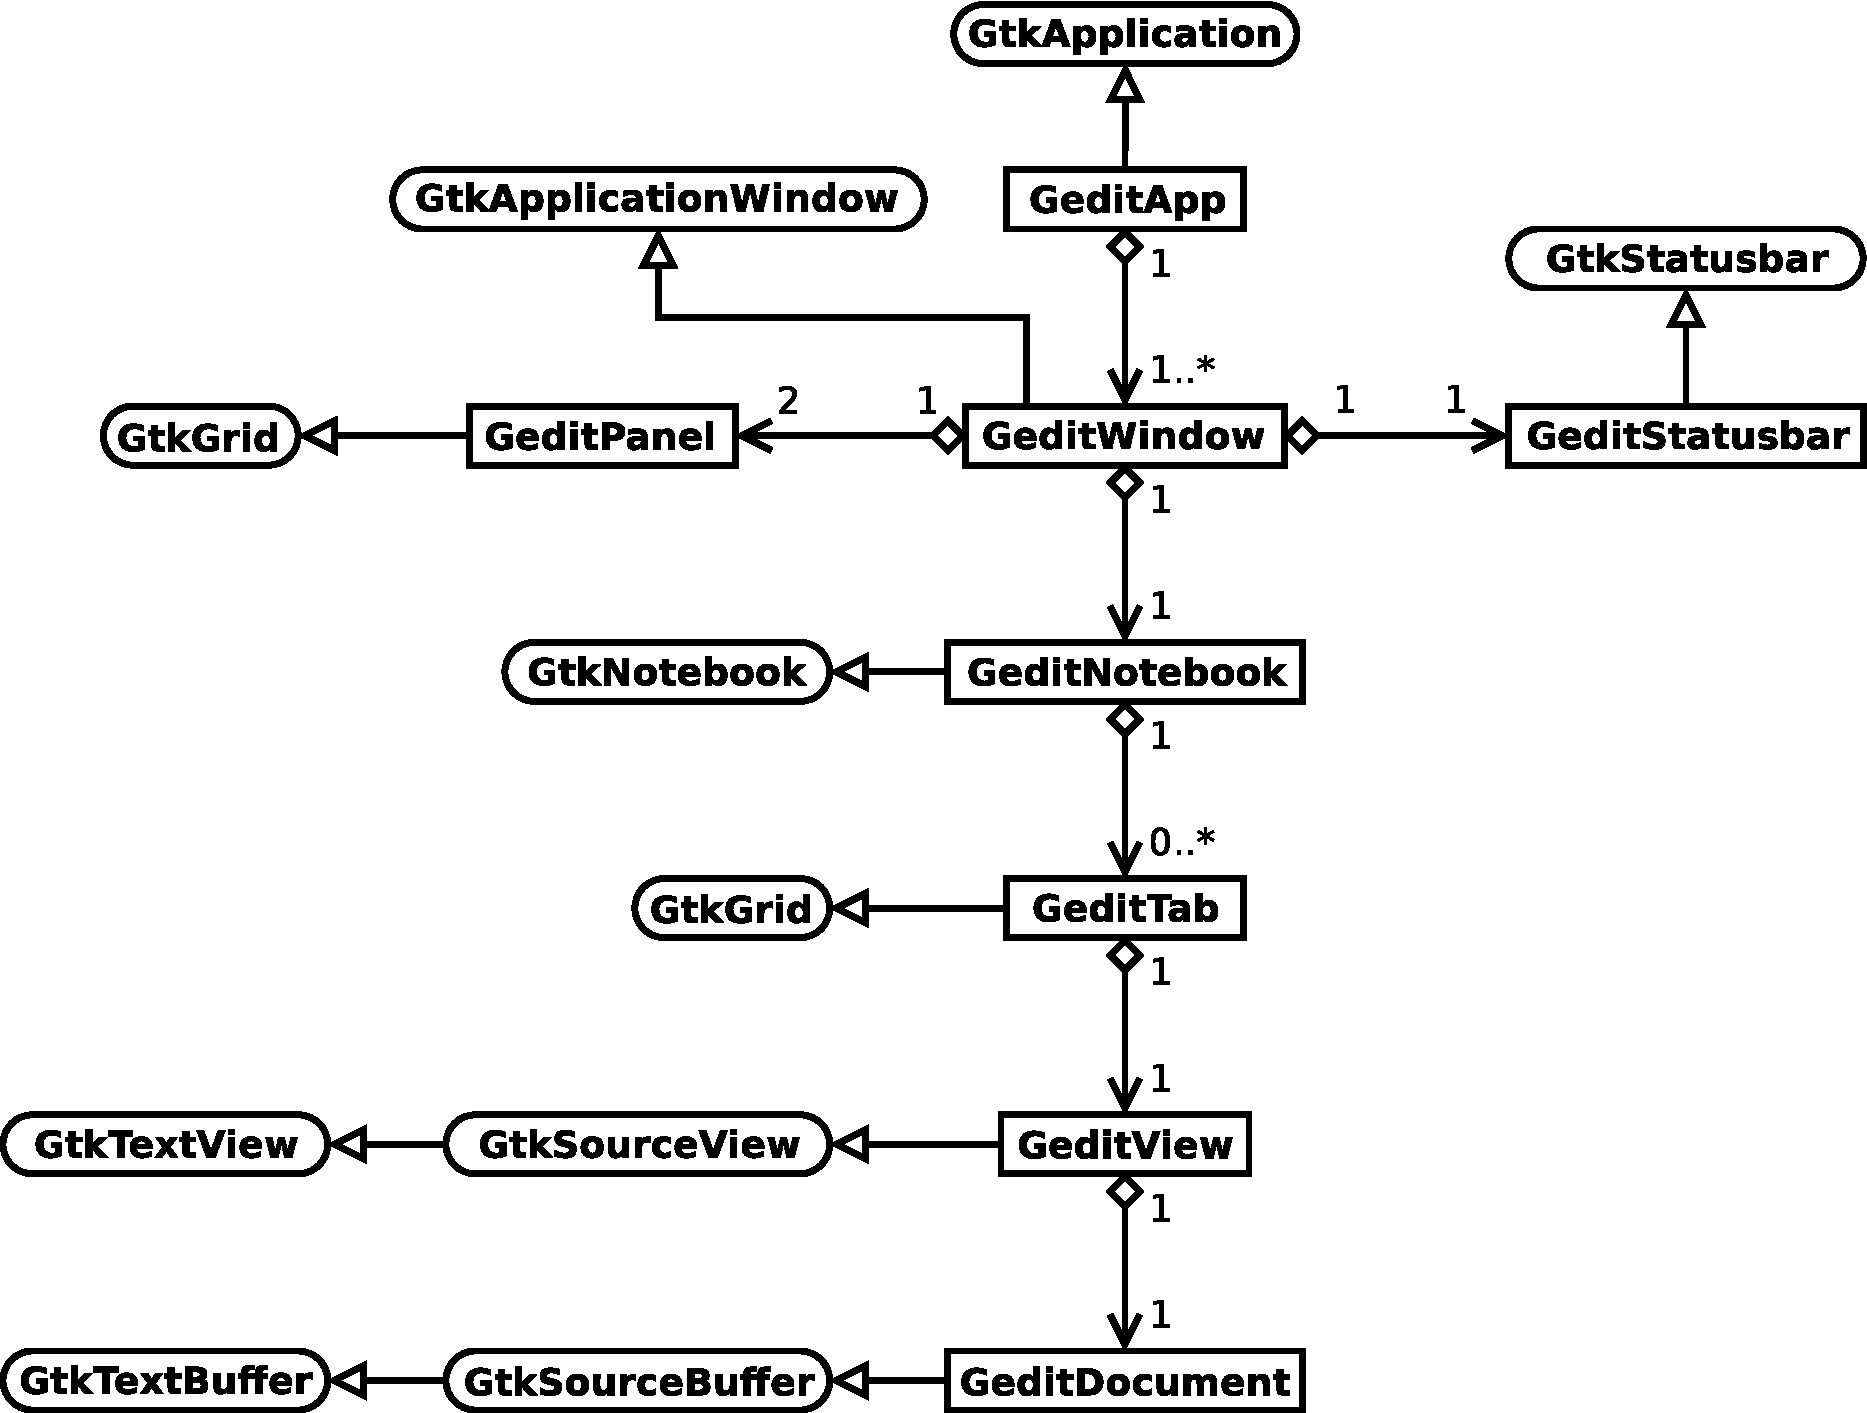
\includegraphics[width=\textwidth]{images/gedit-architecture.pdf}
    \caption{Simplified code architecture of the gedit text editor}
    \label{fig:gedit-architecture}
  \end{center}
\end{figure}

\section{The main() function and GeditApp}

Although not represented on the schema, the entry point of a GTK+ application --~as for every C program~-- is the \lstinline{main()} function. To create a GTK+ application, the principal thing to do in \lstinline{main()} is to create a \lstinline{GtkApplication} instance, or a subclass of it. In the schema we see that \lstinline{GeditApp} is a subclass of \lstinline{GtkApplication}, so the \lstinline{main()} function of gedit creates a \lstinline{GeditApp} object.

\lstinline{GtkApplication} is the class that contains and represents the whole application. There is usually only one instance of \lstinline{GtkApplication} per process, so it can be considered a singleton class. What \lstinline{GtkApplication} contains are the \emph{windows}, for example the \lstinline{GeditWindow}'s in case of gedit, plus other types of windows like dialog windows.

We already saw the \lstinline{GtkApplication} class hierarchy in section~\ref{oop-gobject-inheritance} p.~\pageref{oop-gobject-inheritance} when explaining OOP inheritance with GObject:

\begin{verbatim}
GObject
└── GApplication
    └── GtkApplication
\end{verbatim}

\lstinline{GApplication} is part of the GIO library and implements the features that are not related to the Graphical User Interface (GUI). So for a program that runs in the terminal, it is possible to use \lstinline{GApplication} only.

An important feature that \lstinline{GApplication} provides is process uniqueness (but it can be disabled if not wanted). What process uniqueness does is to have only one process per application per user session. For that feature to work, an application ID must be provided when creating the \lstinline{GApplication} object. With that ID, \lstinline{GApplication} looks if another process already runs the same application in the same user session; if it is the case, it communicates to the primary instance the actions that need to be done (for example opening a new window, or opening a new file in an existing window, etc). When the actions are done on the primary instance, the second process exits immediately. On Linux, \lstinline{GApplication} uses the D-Bus Inter-Process Communication (IPC) system to communicate between the two processes.

Process uniqueness has several advantages, to give a few concrete examples:
\begin{itemize}
  \item For an application with a tabbed document interface, when clicking on a file in a file manager like Nautilus, the file can be opened in a new tab instead of creating each time a new window. For this to work, inter-process communication is needed in one form or another;
  \item An application doesn't need to synchronize explicitly its state and data between different processes. For the sake of argument, let's say that in gedit the user can create custom ``build tools'', to compile the current file or project. gedit saves the custom build tools in an XML file and are shown in the menu to execute their commands. On Linux, the XML file is saved for example in the user's \texttt{\textasciitilde{}/.local/share/} directory. Without process uniqueness, if one gedit process modifies the custom build tools, the other gedit processes need to reload the XML file, and need to ensure that there are no races (two different gedit processes must not modify the XML file at the same time). With process uniqueness, that problem doesn't exist, all the gedit windows share the same application state, and the developer can assume that only one process per user can modify the XML file\footnote{Note that this would not be true if it was possible to open \emph{several} graphical sessions for the same user, on the same machine (with multi-seat support) or at least sharing the backing storage for the home directory (for example with NFS mounts). But GNOME and most applications don't support this, a user can open at most one graphical session at a time for the same home directory. For logins on the same physical machine, this is enforced by GDM (the GNOME display manager and login screen) and D-Bus. For NFS mounts this is not enforced, but if the same user opens several graphical sessions on different computers, some programs might misbehave. So although the \lstinline{GApplication} process uniqueness is documented as being per \emph{user session}, in practice we can say that it is simply per \emph{user}.} (of course the user has still the possibility to edit the XML file by hand, but in that case the application can just be restarted, normally the user is expected to modify the build tools from the GUI that gedit provides).
\end{itemize}

Another important feature of \lstinline{GApplication} is to run the main event loop. The GLib main event loop was described in section~\ref{glib-main-event-loop} p.~\pageref{glib-main-event-loop}. With \lstinline{GApplication}, this is done with the \lstinline{g_application_run()} function. A minimalistic version of the \lstinline{main()} function in gedit would look like:

\begin{lstlisting}
int
main (int    argc,
      char **argv)
{
  GeditApp *app;
  int status;

  /* Init i18n (internationalization) here. */

  app = gedit_app_new ();
  status = g_application_run (G_APPLICATION (app), argc, argv);
  g_object_unref (app);

  return status;
}
\end{lstlisting}

What \lstinline{GeditApp} does is basically what would need to be done in \lstinline{main()} if there was no \lstinline{GtkApplication} subclass. This includes:
\begin{itemize}
  \item Configuring the \lstinline{GtkApplication} object correctly, for example giving the application ID;
  \item Connecting callbacks to some signals\footnote{But note that in a GObject subclass, instead of connecting callbacks to signals of a parent class with e.g. \lstinline{g_signal_connect()}, it is better to override the virtual functions instead.}, for example to create a \lstinline{GeditWindow} when needed;
  \item Implementing application-wide \lstinline{GAction}'s. \lstinline{GAction} is a class part of GIO that represents an action that the user can trigger. An application-wide action is for example to quit the application, or to open the preferences dialog (because the preferences are applied to the whole application).
\end{itemize}

When you start writing a new GTK+ application, you don't see directly the need for a \lstinline{GtkApplication} subclass, since the code in \lstinline{main()}, plus the callbacks, are still small. But when more and more features are added, it is a good idea at some point to move the code to a \lstinline{GtkApplication} subclass. Or to create a subclass directly. A subclass is especially useful when the need arises to store additional data.

\section{GeditWindow}

\lstinline{GeditWindow} is a subclass of \lstinline{GtkApplicationWindow}. And, we don't see it on the schema, but \lstinline{GtkApplicationWindow} is a subclass of \lstinline{GtkWindow}, which is a top-level widget. A top-level widget cannot be contained in another widget. A \lstinline{GtkApplicationWindow} is contained in a \lstinline{GtkApplication}, but \lstinline{GtkApplication} is not a subclass of \lstinline{GtkWidget}.

In the schema, the ``\texttt{1}'' and ``\texttt{1..*}'' notation means that one \lstinline{GeditApp} object \emph{contains} one or several \lstinline{GeditWindow} objects, and that a \lstinline{GeditWindow} is contained in exactly one \lstinline{GeditApp} (a \lstinline{GeditWindow} cannot be contained in several \lstinline{GeditApp} objects, there is anyway only one \lstinline{GeditApp} instance per process).

\lstinline{GeditWindow} is responsible to create the main UI, creating other widgets and assembling them in a \lstinline{GtkGrid} container for example. Another thing that \lstinline{GeditWindow} does is to implement the \lstinline{GActions} that have an effect only on the current window, for example an action to close the window, or save the current document. When implementing a \lstinline{GAction}, \lstinline{GeditWindow} can of course delegate most of its work to other classes contained in \lstinline{GeditWindow}.

At the top of a main application window, there is usually a \lstinline{GtkHeaderBar}, that shows the window title, some buttons and an ``hamburger'' menu. Alternatively, an application can have a traditional menubar and toolbar.

Besides the headerbar, \lstinline{GeditWindow} creates a \lstinline{GeditStatusbar} widget and adds it to the bottom of the window. It also creates two \lstinline{GeditPanels}, one on the left side of the window, and the other on the bottom, above the \lstinline{GeditStatusbar}. Each panel can contain several elements. For example the side panel contains an integrated file browser, and the bottom panel can contain a terminal, among other things\footnote{The current gedit code actually doesn't contain a \lstinline{GeditPanel} class anymore, but it was the case in an earlier version. Adding \lstinline{GeditPanel} to the diagram was done to show a possible implementation of panels in an application. If your application contains only one element in a panel, no need to have a \lstinline{Panel} class, you can directly add the element to the window.}.

\lstinline{GeditWindow} also creates a \lstinline{GeditNotebook}, the main part of the window.

\section{GeditNotebook and What It Contains}

\lstinline{GeditNotebook} is a subclass of \lstinline{GtkNotebook}, which is the widget that displays tabs, and also contains their content.

In the class schema, we can see that the content of a tab is a \lstinline{GeditTab} widget, a subclass of \lstinline{GtkGrid}. The main element inside a \lstinline{GeditTab} is the \lstinline{GeditView}. More precisely --- it was omitted in the schema for succinctness --- the \lstinline{GeditView} is actually contained in a \lstinline{GtkScrolledWindow} which is contained in the \lstinline{GeditTab}. But \lstinline{GeditTab} can contain other widgets, for example information bars on top of the document.

\lstinline{GeditView} is a subclass of \lstinline{GtkSourceView}, which is itself a subclass of \lstinline{GtkTextView}. \lstinline{GtkTextView} --- which is part of GTK+ --- is the foundation for a multiline text editor. The GtkSourceView library adds features useful for source code, such as syntax highlighting. \lstinline{GtkTextView} follows a Model-View-Controller pattern. \lstinline{GtkTextBuffer} is the model, i.e. it contains the data.

\section{Why and When Creating Sub-Classes of GTK+ Widgets?}

If we look for instance at \lstinline{GeditTab}, it contains --- by composition --- a \lstinline{GeditView}. \lstinline{GeditView} is a subclass of \lstinline{GtkSourceView}. Instead, \lstinline{GeditTab} could use by composition directly a \lstinline{GtkSourceView} object, and move the code of \lstinline{GeditView} to \lstinline{GeditTab}. But usually, it's exactly the opposite that happens or should happen.

When a GTK+ application codebase is still small, for example if you start writing an equivalent of \lstinline{GeditTab}, you can create a \lstinline{GtkSourceView} object directly in \lstinline{GeditTab}, and store the \lstinline{GtkSourceView} object in an instance variable. Then, when implementing new features, you add new functions that use almost exclusively the \lstinline{GtkSourceView} instance variable. You may even have \lstinline{static} functions that take directly a \lstinline{GtkSourceView} argument instead of the \lstinline{GeditTab} \emph{self} parameter. You may also store additional data useful only to the \lstinline{GtkSourceView}-related functions. If the \lstinline{GeditTab} class is still small (e.g. 500 lines of code) and doesn't contain a lot of instance variables, there is no problem. On the other hand, if the \lstinline{GeditTab} class becomes larger (e.g. more than 2000 lines of code), then it's probably a sign that the class should delegate some of its work to a new class; in our case, \lstinline{GeditView}. Note that 2000 lines of code for a class might be fine, there is no clear boundary on when a class should be split. But if the resulting \lstinline{GeditView} class would contain at least several hundreds of non-boilerplate code, it is probably a good idea to do the refactoring.

What OOP is all about is to pack data and behavior together, and delegate some of the work to other classes. Class inheritance makes sense when we want to add more behavior to an existing class, with possible additional data related to the added behavior. \lstinline{GeditView} is a subclass of \lstinline{GtkSourceView} because \lstinline{GeditView} \emph{is~a} \lstinline{GtkSourceView}; that is, \lstinline{GeditView} operates on the same base data as \lstinline{GtkSourceView}. In addition, it permits to \lstinline{GeditTab} to delegate some of its work, with the goal to have smaller, more manageable classes. Smaller in two ways: less code, and less instance variables.

So, during the lifetime of a GTK+ application, the programmer often needs to refactor the code, creating new classes, delegating more work. The opposite can happen when application code is moved to the underlying library; for example, if all the features of \lstinline{GeditView} are added to the \lstinline{GtkSourceView} class; in that case, the \lstinline{GeditView} subclass doesn't make sense anymore.

\section{Composite Widgets}

Composite widgets are containers that already contain a useful collection of child widgets in a nice package. Implementing a composite widget is easy\footnote{Once you know how to subclass a GObject class.}, you just need to:
\begin{enumerate}
  \item Subclass a container like \lstinline{GtkGrid} or \lstinline{GtkBin} or \lstinline{GtkWindow};
  \item In the constructor of the class, create the child widgets and add them to the container.
\end{enumerate}

In the gedit class schema, the composite widgets are the subclasses of \lstinline{GtkGrid} (\lstinline{GeditPanel} and \lstinline{GeditTab}) and \lstinline{GeditWindow}.

\lstinline{GeditWindow} is an indirect subclass of \lstinline{GtkBin}, so it can contain at most one child widget. That's why \lstinline{GeditWindow} uses a \lstinline{GtkGrid} as its child widget, so that the \lstinline{GtkGrid} can contain in turn all the window elements.

By default a \lstinline{GeditTab} has only one child widget, the \lstinline{GtkScrolledWindow} that contains the \lstinline{GeditView}. But \lstinline{GeditTab} has a function to add a \lstinline{GtkInfoBar} at the top, showing for example an error message.

So, while \lstinline{GtkGrid} is a general-purpose container that doesn't contain any child widget initially, a composite widget is a specialized container that already contains specific child widgets. Writing composite widgets are a convenient way to code applications.

%TODO show code example

\chapter{Further Reading}
\label{further-reading}

At this point you should know the basics of GLib core and GObject. You don't need to know \emph{everything} about GLib core and GObject to continue, but having at least a basic understanding will allow you to more easily learn GTK+ and GIO, or any other GObject-based library for that matter.

\section{GTK+ and GIO}
GTK+ and GIO can be learned in parallel.

You should be able to use any GObject class in GIO, just read the class description and skim through the list of functions to have an overview of what features a class provides. Among other interesting things, GIO includes:
\begin{itemize}
  \item \lstinline{GFile} to handle files and directories.
  \item \lstinline{GSettings} to store application settings.
  \item \lstinline{GDBus} -- a high-level API for the D-Bus inter-process communication system.
  \item \lstinline{GSubprocess} for launching child processes and communicate with them asynchronously.
  \item \lstinline{GCancellable}, \lstinline{GAsyncResult} and \lstinline{GTask} for using or implementing asynchronous and cancellable tasks.
  \item Many other features, like I/O streams, network support or application support.
\end{itemize}

For building graphical applications with GTK+, don't panic, the reference documentation has a Getting Started guide, available with Devhelp or online at:\\
\url{https://developer.gnome.org/gtk3/stable/}

After reading the Getting Started guide, skim through the whole API reference to get familiar with the available widgets, containers and base classes. Some widgets have a quite large API, so a few external tutorials are also available, for example for \lstinline{GtkTextView} and \lstinline{GtkTreeView}. See the documentation page on:\\
\url{http://www.gtk.org}

There is also a series of small tutorials on various GLib/GTK+ topics:\\
\url{https://wiki.gnome.org/HowDoI}

\section{Autotools}

A Makefile is generally not sufficient if you want to install your application on different systems. The Autotools (Autoconf, Automake and Libtool) are what GNOME modules use. Macros are available for various purposes (the user documentation, code coverage statistics for unit tests, etc.). The most recent book on the subject is \emph{Autotools}, by John~Calcote \cite{autotools}.

\section{Programming Best-Practices}

It is recommended to follow the GNOME Programming Guidelines~\cite{gnome-programming-guidelines}.

The following list is a bit unrelated to GLib/GTK+ development, but is useful for any programming project. After having some practice, it is interesting to learn more about programming \emph{best}-practices. Writing code of good quality is important for preventing bugs and for maintaining a piece of software in the long-run.

\begin{itemize}
  \item \emph{The} book on programming best-practices is \emph{Code Complete}, by Steve~McConnell \cite{code-complete}. Highly recommended\footnote{Although the editor of \emph{Code Complete} is Microsoft Press, the book is not related to Microsoft or Windows. The author sometimes explains stuff related to open source, UNIX and Linux, but one can regret the total absence of the mention ``free/libre software'' and all the benefits of freedom, in particular for this kind of book: being able to learn by reading other's code. But if you are here, you hopefully already know all of this.}.

  \item For guidelines about OOP specifically, see \emph{Object-Oriented Design Heuristics}, by Arthur~Riel \cite{oop-book}.

  \item An excellent source of information is the website of Martin~Fowler: refactoring, agile methodology, code design, ...\\
  \url{http://martinfowler.com/}
\end{itemize}

More related to GNOME, Havoc~Pennington's articles have good advice worth the reading, including ``\emph{Working on Free Software}'', ``\emph{Free software UI}'' and ``\emph{Free Software Maintenance: Adding Features}'':\\
\url{http://ometer.com/writing.html}

\begin{thebibliography}{10}
\addcontentsline{toc}{chapter}{Bibliography}

\bibitem{k-r-book}
Brian \textsc{Kernighan} and Dennis \textsc{Ritchie},
\emph{The C Programming Language},
Second Edition, Prentice Hall, 1988.

\medskip
\bibitem{oop-book}
Arthur \textsc{Riel},
\emph{Object-Oriented Design Heuristics},
Addison-Wesley, 1996.

\medskip
\bibitem{algo-book}
Steven \textsc{Skiena},
\emph{The Algorithm Design Manual},
Second Edition, Springer, 2008.

\medskip
\bibitem{unix-impatient}
Paul \textsc{Abrahams},
\emph{UNIX for the Impatient},
Second Edition, Addison-Wesley, 1995.

\medskip
\bibitem{pro-git}
Scott \textsc{Chacon},
\emph{Pro Git},
\url{https://git-scm.com/book}

\medskip
\bibitem{autotools}
John \textsc{Calcote},
\emph{Autotools -- A Practitioner's Guide to GNU Autoconf, Automake, and Libtool},
No Starch Press, 2010.

\medskip
\bibitem{code-complete}
Steve \textsc{McConnell},
\emph{Code Complete -- A practical handbook of software construction},
Second Edition, Microsoft Press, 2004.

\medskip
\bibitem{gtk-doc}
\emph{GTK-Doc Manual},
\url{https://developer.gnome.org/gtk-doc-manual/}

\medskip
\bibitem{gobject-introspection}
\emph{GObject Introspection},\\
\url{https://wiki.gnome.org/Projects/GObjectIntrospection}

\medskip
\bibitem{gnome-programming-guidelines}
\emph{GNOME Programming Guidelines},\\
\url{https://developer.gnome.org/programming-guidelines/stable/}

\end{thebibliography}


\end{document}
